\documentclass{article}
\usepackage{listings}                                           %插入代码
\usepackage{geometry}                                           %设置页面大小边距等
\usepackage{graphicx}                                           %插入图片
\usepackage{amssymb}                                            %为了用\mathbb
\usepackage{amsmath}                                            %数学方程的显示
\usepackage{listings}                                           %插入代码
\usepackage{fancyhdr}                                           %设置页眉页脚
\usepackage{lastpage}                                           %总页数
\usepackage{hyperref}                                           %引用网页
\usepackage{xcolor}
\usepackage{tikz}
\usepackage{float}
\usepackage{subcaption} 
\usepackage{mathrsfs}
\bibliographystyle{unsrt}



\geometry{a4paper,left=2cm,right=2cm,top=2cm,bottom=2cm}        %一定要放在前面!
\pagestyle{fancy}                                               %设置页眉页脚
\lhead{Guanyu Chen}                                       %页眉左Fir                                        

\rhead{SDEs}                                                %章节信息
\cfoot{\thepage/\pageref{LastPage}}                             %当前页,记得调用前文提到的宏包
\lfoot{Zhejiang University}
\rfoot{College Of Integrated Circuits}
\renewcommand{\headrulewidth}{0.1mm}                            %页眉线宽,设为0可以去页眉线
\renewcommand{\footrulewidth}{0.1mm}                            %页脚线宽,设为0可以去页眉线
\setlength{\headwidth}{\textwidth}

\hypersetup{                                                    %设置网页链接颜色等
    colorlinks=true,                                            %链接将会有颜色,默认是红色
    linkcolor=red,                                             %内部链接,那些由交叉引用生成的链接将会变为蓝色(blue)
    filecolor=red,                                          %链接到本地文件的链接将会变为洋红色(magenta)
    urlcolor=red,      
    citecolor=black                                       
}

\lstset{  
    basicstyle=\ttfamily,  
    keywordstyle=\color{blue},  
    language=Python,  
    numbers=left,  
    numberstyle=\tiny\color{gray},  
    frame=single,  
    breaklines=true  
}  

\newtheorem{theorem}{Theorem}
\newtheorem{proof}{Proof}
\newtheorem{solution}{Solution:}
\newtheorem{remark}{Remark}
\newtheorem{definition}{Definition}
\newtheorem{algorithm}{Algorithm}
\newtheorem{lemma}{Lemma}
\newtheorem{problem}{Problem}
\newtheorem{example}{Example}

\title{Stochastic Differential Equations}
\author{Guanyu Chen}
\date{\today}
\begin{document}
\maketitle
\begin{abstract}
    This paper is about the basic theory and applications of SDEs. Also, this is a sum up of last term's SDE course. Reference: \cite{song2021scorebasedgenerativemodelingstochastic}\cite{chan2024tutorialdiffusionmodelsimaging}\cite{citeulike:1220946}
    \cite{lipman2024flowmatchingguidecode}\cite{lord2014introduction}\cite{Särkkä_Solin_2019}\cite{holderrieth2023fokker} \cite{doi:10.1137/1.9780898718997}
    
\end{abstract}
\tableofcontents
\newpage
\section{Introduction to SDEs}
\subsection{SODEs}
\begin{problem}
    Assume we have a Stochastic Differential Equation like:
    \begin{equation}\label{sde}
        dX_t = f(X_t, t)dt + G(X_t, t)dW_t
    \end{equation}
    where $X_t\in \mathbf{R}^d,f\in \mathcal{L}(\mathbf{R}^{d+1}, \mathbf{R}^d)$, and $W_t$ is m-dim Brownian Motion with diffusion matrix $Q$, 
    $G(X_t, t)\in \mathcal{L}(\mathbf{R}^{m+1}, \mathbf{R}^d)$, with initial condition $X_0\sim p(X_0)$.
\end{problem}
\subsection{The It'so and Stratonovich Stochastic Integrals}
\subsection{Ito's Formula}

\subsection{Mean and Covariance}
We can derive the mean and covariance of SDE.
By applying Ito's formula to $\phi(x, t)$, then
\begin{equation}
    \frac{d E[\phi]}{d t}=E\left[\frac{\partial \phi}{\partial t}\right]+\sum_{i} E\left[\frac{\partial \phi}{\partial x_{i}} f_{i}(X_t, t)\right]+\frac{1}{2} \sum_{i j} E\left[\frac{\partial^{2} \phi}{\partial x_{i} \partial x_{j}}\left[G Q G^{\top}\right]_{i j}\right]
\end{equation}
By taking $\phi(X, t)=x_i$ and $\phi(X, t)=x_ix_j-m(t)_im(t)_j$, we have the mean function $m(t)=E[X_t]$ 
and covariance function $c(t)=E\left[\left(X_t-m(t)\right)\left(X_t-m(t)\right)^T\right]$ respectively, s.t.
\begin{equation}\label{SDEMC}
    \left\{
        \begin{aligned}
            &\frac{d m}{d t}=E\left[f(X_t, t)\right]\\
            &\frac{d c}{d t}=E\left[f(X, t)(X-m(t)^T)\right]+E\left[(X-m(t)f^T(X, t))\right]+E\left[G(X_t, t)QG^T(X_t, t)\right]
        \end{aligned}
    \right.
\end{equation}
So we can estimate the mean and covariance of solution to SDE. However, these equations cannot be used as such, 
because only in the Gaussian case do the expectation and covariance actually characterize the distribution. 

The linear SDE has explicit solution. Assume the linear SDe has the form 
\begin{equation}
    dX_t =\left(K(t)X_t + B(t)\right)dt + G(t)dW_t
\end{equation}
where $K(t)\in \mathbf{R}^{d\times d}, B(t)\in \mathbf{R}^{d}, G(t)\in \mathbf{R}^{d\times m}$ are given functions. 
$X_t \in \mathbf{R}^d$ is the state vector, $W_t \in \mathbf{R}^m$ is the Brownian Motion with diffusion matrix $Q$.

\begin{theorem}
    The explicit solution to the linear SDE is given by:
    \begin{equation}\label{explicitsolLSDE}
        X_t = \Psi(t, t_0)X_0 + \int_{t_0}^t \Psi(t, s)B(s)ds + \int_{t_0}^t \Psi(t, s)G(s)dW_s
    \end{equation}
    where $\Psi(t, t_0)$ is the transition matrix of the linear SDE, which satisfies the following matrix ODE:
    \begin{equation}
        \frac{d\Psi}{dt} = K(t)\Psi(t, t_0), \Psi(t_0, t_0) = I
    \end{equation}
    Hence, $X_t$ is a Gaussian process(A linear transformation of Brownian Motion which is a Gaussian process).
\end{theorem}
\begin{proof}
    Multiply both sides of the SDE by Integrating factor $\Psi(t_0, t)$ and apply Ito's formula to $\Psi(t_0, t)X_t$.

    See Sarkka P49.
\end{proof}
As discussed above, we can compute the mean and covariance function of solution to linear SDE. 
\begin{theorem}
    The mean and covariance function of solution to linear SDE are given by:
    \begin{equation}
        \left\{
            \begin{aligned}
                &\frac{d m}{d t} = K(t)m(t) + B(t)\\
                &\frac{d c}{d t} = K(t)c(t) + c(t)K^T(t)+ G(t)QG^T(t)
            \end{aligned}
        \right.
    \end{equation}
    with initial condition $m_0 =m(t_0)=E[X_0], c_0 =c(t_0)=Cov(X_0)$. Then the solution is given by solving the above ODEs:
    \begin{equation}\label{LSDEMC}
        \left\{
            \begin{aligned}
                &m(t) = \Psi(t, t_0)m_0 + \int_{t_0}^t \Psi(t, s)B(s)ds\\
                &c(t) = \Psi(t, t_0)c_0\Psi^T(t, t_0) + \int_{t_0}^t \Psi(t, s)G(s)QG^T(s)\Psi^T(t, s)ds
            \end{aligned}
        \right.
    \end{equation}

\end{theorem}
\begin{proof}
    Apply $F(X, t)=K(t)X + B(t), G(X, t)=G(t)$ to \ref{SDEMC}.
\end{proof}

Hence the solution to linear SDE is a Gaussian process with mean and covariance function given by the above ODEs.
\begin{theorem}
The solution to LSDE is Gaussian:
\begin{equation}
    p(X, t) = \mathcal{N}(X(t)|m(t), c(t))
\end{equation}
Specially when $X_0 = x_0$ is fixed, then 
\begin{equation}\label{transitiondensity}
    p(X,t|X_0=x_0) = \mathcal{N}(X(t)|m(t|x_0), c(t|x_0))
\end{equation}
That is, $m_0 = x_0, c_0 = 0$. Then we have:
\begin{equation}
    \left\{
        \begin{aligned}
            &m(t|x_0) = \Psi(t, t_0)x_0 + \int_{t_0}^t \Psi(t, s)B(s)ds\\
            &c(t|x_0) = \int_{t_0}^t \Psi(t, s)G(s)QG^T(s)\Psi^T(t, s)ds
        \end{aligned}
    \right.
\end{equation}
\end{theorem}
\begin{proof}
    The proof is straight foward either by applying $m_0 = x_0, c_0 = 0$ to \ref{LSDEMC} or by eq \ref{explicitsolLSDE}.
\end{proof}
So, to sum up, linear SDE has great properties! The distribution is completedly decided by the inital condition.
Also, if we generate $X_0$ to $X_{t_k}$, which means that we begin SDE at $t_i$ with $X_{t_i}$, we have the equivalent discretization of SDE:
\begin{theorem}
    Original SDE is weakly, in distribution, equivalent to the following discrete-time SDE:
    \begin{equation}\label{DTSDE}
        X_{t_{i+1}} = A_iX_{t_i} + B_i + G_i
    \end{equation} 
    where
    \begin{equation}\left\{
        \begin{aligned}
            A_i &= \Psi(t_{i+1}, t_i)\\
            B_i &= \int_{t_i}^{t_{i+1}} \Psi(t_{i+1}, s)B(s)ds\\
            G_i &= \int_{t_i}^{t_{i+1}} \Psi(t_{i+1}, s)G(s)QG^T(s)\Psi^T(t_{i+1}, s)ds
        \end{aligned}\right.
    \end{equation}
\end{theorem}
\begin{proof}
    The proof is straight forward.
\end{proof}
\begin{theorem}
    The covariance of $X_t$ and $X_s(s<t)$ is given by:
    \begin{equation}
        Cov(X_t, X_s) = \Psi(t, s)c(s)
    \end{equation}
\end{theorem}

\begin{proof}
    See Sarkka P88-89.
\end{proof}




\section{Fokker-Planck-Kolmogorov Equation}
\subsection{FPK Equation}
\begin{definition}[Generator]
    The infinitesimal generator of a stochastic process $X(t)$ for function $\phi(x)$, i.e. $\phi(X_t)$ can be defined as
    \begin{equation}
        \mathcal{A} \phi(X_t)=\lim _{s \rightarrow 0^{+}} \frac{E[\phi(X(t+s)]-\phi(X(t))}{s}
    \end{equation}
    Where  $\phi$  is a suitable regular function.
\end{definition}
This leads to Dynkin's Formula very naturally.
\begin{theorem}[Dynkin's Formula]
    \begin{equation}
        E[f(X_t)]=f(X_0)+E\left[\int_0^t\mathcal{A}(f(X_s))ds\right]
    \end{equation}
\end{theorem}

\begin{theorem}
    If  $X(t)$  s.t. \ref{sde}, then the generator is given:
\begin{equation}
    \mathcal{A}(\cdot)=\sum_{i} \frac{\partial(\cdot)}{\partial x_{i}} f_{i}(X_t, t)+\frac{1}{2} \sum_{i, j}\left(\frac{\partial^{2}(\cdot)}{\partial x_{i} \partial x_{j}}\right)\left[G(X_t, t)Q G^{\top}(X_t, t)\right]_{i j}
\end{equation}
\end{theorem}
\begin{proof}
    See P119 of SDE by Oksendal.
\end{proof}

\begin{example}
    If $dX_t=dW_t$, then $\mathcal{A}=\frac{1}{2}\Delta$, where $\Delta$ is the Laplace operator.
\end{example}

\begin{definition}[Generalized Generator]
    For $\phi(x, t)$, i.e. $\phi(X_t, t)$, the generator can be defined as:
    \begin{equation}
        A_{t} \phi(x, t)=\lim _{s \rightarrow 0^{+}} \frac{E[\phi(X(t+s), t+s)]-\phi(X(t), t)}{s}
    \end{equation}
\end{definition}

\begin{theorem}
    Similarly if $X(t)$ s.t. \ref{sde}, then the generalized generator is given:
    \begin{equation}
        \mathcal{A}_t(\cdot)=\frac{\partial(\cdot)}{\partial t}+\sum_{i} \frac{\partial(\cdot)}{\partial x_{i}} f_{i}(X_t, t)+\frac{1}{2} \sum_{i, j}\left(\frac{\partial^{2}(\cdot)}{\partial x_{i} \partial x_{j}}\right)\left[G(X_t, t) Q G^{\top}(X_t, t)\right]_{i j}
    \end{equation}
\end{theorem}
We want to consider the density distribution of $X_t, P(x, t)$
\begin{theorem}[Fokken-Planck-Kolmogorov equation]
    The density function $P(x, t)$ of $X_t$ s.t. \ref{sde} solves the PDE:
    \begin{equation}
        \frac{\partial P(x, t)}{\partial t}=-\sum_{i} \frac{\partial}{\partial x_{i}}\left[f_{i}(x, t) p(x, t)\right]+\frac{1}{2} \sum_{i, j} \frac{\partial^{2}}{\partial x_{i} \partial x_{j}}\left[\left(G Q G^{\top}\right)_{i j} P(x, t)\right]
    \end{equation}
    The PDE is called FPK equation / forwand Kolmogorov equation.
\end{theorem}
\begin{proof}
    Consider the function $\phi(x)$, let $x=X_t$ and apply Ito's Formula:
    \begin{equation}
        \begin{aligned}
            d \phi & =\sum_{i} \frac{\partial \phi}{\partial x_{i}} d x_{i}+\frac{1}{2} \sum_{i, j}\left(\frac{\partial^{2} \phi}{\partial x_{i} \partial x_{j}}\right) d x_{i} d x_{j} \\
            & =\sum_{i} \frac{\partial \phi}{\partial x_{i}}\left(f_{i}\left(X_t, t\right) d t+\left(G\left(X_{t}, t\right) d W_{t}\right)\right)+\frac{1}{2} \sum_{i, j}\left(\frac{\partial^{2} \phi}{\partial x_{i} \partial x_{j}}\right)\left[G(X_t, t) Q G^{\top}(X_t, t)\right]_{i j} d t .
            \end{aligned}
    \end{equation}
    Take expectation of both sides:
    \begin{equation}\label{expectation}
        \frac{d E[\phi]}{d t}=\sum_{i} E\left[\frac{\partial \phi}{\partial x_{i}} f_{i}(X_t, t)\right]+\frac{1}{2} \sum_{i j} E\left[\frac{\partial^{2} \phi}{\partial x_{i} \partial x_{j}}\left[G Q G^{\top}\right]_{i j}\right]
    \end{equation}
    So 
    \begin{equation}\left\{
        \begin{aligned}
            &\frac{d E[\phi]}{d t} =\frac{d}{d t}\left[\int \phi(x) P(X_t=x, t) d x\right]=\int \phi(x) \frac{\partial P(x, t)}{\partial t} dx\\
            &\sum_{i} E\left[\frac{\partial \phi}{\partial x_{i}} f_{i}\right]=\sum_{i} \int\frac{\partial \phi}{\partial x_{i}} f_{i}(X_t=x, t) P d x
            =-\sum_{i} \int \phi \cdot \frac{\partial}{\partial x_{i}}\left[f_{i}(x, t) p(x, t)\right] d x . \\
            &\frac{1}{2} \sum_{i j} E\left[\frac{\partial^{2} \phi}{\partial x_{i} \partial x_{j}}\left[G Q G^{\top}\right]_{i j}\right]=\frac{1}{2} \sum_{i j} \int \frac{\partial^{2} \phi}{\partial x_{i} \partial x_{j}}\left[G Q G^{\top}\right]_{i j} P d x
            =\frac{1}{2} \sum_{i j} \int \phi(x) \frac{\partial^{2}}{\partial x_{i} \partial x_{j}}\left(\left[G Q G^{\top}\right]_{i j} P\right) d x. \\
        \end{aligned}\right.
    \end{equation}
    then
    $$\int \phi  \frac{\partial P}{\partial t} d X=-\sum_{i} \int \phi  \frac{\partial}{\partial x_{i}}\left(f_{i} P\right) d X+\frac{1}{2} \sum_{i j} \int \phi \frac{\partial^{2}}{\partial x_{i} x_{j}}\left(\left[G Q G^{\top}\right]_{i j} P\right) d x$$
    Hence $$\int \phi \cdot\left[\frac{\partial P}{\partial t}+\sum_{i} \frac{\partial}{\partial x_{i}}\left(f_{i} P\right)-\frac{1}{2} \sum_{i j} \frac{\partial^{2}}{\partial x_{i} \partial x_{j}}\left(\left[G Q G^{\top}\right]_{i j} P\right)\right] d X=0$$
    Therefore P s.t.    
    \begin{equation}
        \frac{\partial P}{\partial t}+\sum_{i} \frac{\partial}{\partial x_{i}}\left(f_{i}(x, t) P(x, t)\right)-\frac{1}{2} \sum_{i=1} \frac{\partial^{2}}{\partial X_{i} \partial X_{j}}\left(\left[G Q G^{\top}\right]_{i j} P\left(x,t\right)\right)=0
    \end{equation}
    Which gives the FPK Equation.
\end{proof}

\begin{remark}
    When SDE is time independent:  
    \begin{equation}
        d X_t=f(X_t) d t+G(X_t) d W_{t}  
    \end{equation}
    then the solution of FPK often converges to a stationary solution s.t.  $\frac{\partial P}{\partial t}=0$.
\end{remark}
Here is an another way to show FPK equation: Since we have inner product $\langle\phi, \psi\rangle=\int \phi(x)\psi(x)dx$. Then $E[\phi(x)]=\langle\phi, P\rangle$.

As the equation \ref{expectation} can be written as 
\begin{equation}
    \frac{d}{dt}\langle\phi, P\rangle=\langle\mathcal{A}\phi, P\rangle
\end{equation}
Where $\mathcal{A}$ has been mentioned above. If we note the adjoint operator of $\mathcal{A}$ as $\mathcal{A}^*$, then we have
\begin{equation}
    \langle\phi, \frac{dP}{dt}-\mathcal{A}^*(P)\rangle=0,\forall \phi(x)
\end{equation}
Hence we have 
\begin{theorem}[FPK Equation]
    \begin{equation}
    \frac{dP}{dt}=\mathcal{A}^*(P),\operatorname{where} \mathcal{A}^*(\cdot)=-\sum_{i} \frac{\partial}{\partial x_{i}}\left(f_{i}(x, t) (\cdot)\right)+\frac{1}{2} \sum_{i=1} \frac{\partial^{2}}{\partial x_{i} \partial x_{j}}\left(\left[G Q G^{\top}\right]_{i j}(\cdot)\right)
\end{equation}
It can be rewritten as:
\begin{equation}
    \begin{aligned}
        \frac{\partial P}{\partial t} &= -\nabla\cdot\left[f(x, t) P(x, t)\right]+\frac{1}{2} \nabla^2\cdot\left[\left(G Q G^{\top}\right) P(x, t)\right] \\
        &=-\nabla\cdot\left[f(x, t) P(x, t)-\frac{1}{2} \nabla\cdot\left[\left(G Q G^{\top}\right) P(x, t)\right]\right]
    \end{aligned}
\end{equation}

We define the probability flux to be:
\begin{equation}
    J(x, t) = f(x, t) p(x, t)-\frac{1}{2} \nabla\cdot\left[M(x) p(x, t)\right], M(x)=G(x, t)Q(x, t)G(x, t)^T
\end{equation}
Integrating the Fokker-Planck equation over $\mathbb{R}^d$ and using the divergence theorem on the right hand side of  the equation, we have:
\begin{equation}
    \frac{d}{dt}\int_{R^d}p(x, t)dx=\int_{R^d}\nabla\cdot J(x, t)dx=0
\end{equation}
The stationary Fokker-Planck equation, whose solutions give us the invariant distributions of the diffusion process $X_t$, can be written in the form
\begin{equation}
    \nabla \cdot J(x, t)=0
\end{equation}
Consequently, the equilibrium probability flux is a divergence-free vector field.

\end{theorem}

\subsection{Forward and backward Komogorov Equation}
\begin{theorem}
    Fix $t>s$, let $u(x, s):= E\left[g(X_t)|X_s=x\right]=\int g(y)P(y, t|x, s)dy$, then $u(x, s)$ satisfies the following equation:
    \begin{equation}
        \frac{\partial u}{\partial s}+f(x, s)\cdot \nabla u+\frac{1}{2}\nabla \cdot (M\nabla u)=0, \qquad u(x, s)=g(x)
    \end{equation}
\end{theorem}

\begin{theorem}[Transition Density(Forward Komogorov Equation)]
     The transition density $P_{t|s}(x_t|x_s),t\geq s$, which means the propability of transition from $X(s)=x_s$ to $X(t)=x_t$, satisfies the FPK equation with initial condition $P_{s|s}(x|x_s)=\delta(x-x_s)$
     i.e. for $P_{t|s}(x|y)$, it solves
     \begin{equation}
        \frac{\partial P_{t|s}(x|y)}{\partial t}=\mathcal{A}^*(P_{t|s}(x|y)), \operatorname{with} P_{s|s}(x|y)=\delta(x-y)
     \end{equation}
\end{theorem}




\subsection{Ornstein-Uhlenbeck Process}
\begin{definition}[Ornstein-Uhlenbeck Process]
    The Ornstein-Uhlenbeck Process is defined as:
    \begin{equation}
        dX_t = -\alpha X_t dt+\sqrt{2D} dW_t
    \end{equation}
    where $\alpha>0, D>0$, normally $D = \frac{1}{\beta}$.
\end{definition}
By FPK equation, we have:
\begin{equation}\left\{
    \begin{aligned}
        &\frac{\partial p}{\partial t} = \alpha \frac{\partial}{\partial x}(xp)+D\frac{\partial^2 p}{\partial x^2}\\
        &p_{0}(x|x_0) = \delta(x-x_0)
    \end{aligned}\right.\label{OU}
\end{equation}
When (\ref{OU}) is  used to model the velocity or position of a particle, the noisy term on the right hand side of the equation is related to thermal fluctuations.
The solution of (\ref{OU}) can be computed:
\begin{equation}
    X_t \sim N(x_0e^{-\alpha t}, \frac{D}{\alpha}(1-e^{-2\alpha t}))
\end{equation}
The generator of OU process is:
\begin{equation}
    \mathcal{L}=-\alpha x\cdot \nabla +D\Delta
\end{equation}

We need to study the properties of the generator $\mathcal{L}$. When the unique invariant density of OU is $\rho$, do transformation:
\begin{equation}
    \mathcal{L}^*(h\rho)=\rho \mathcal{L}h
\end{equation}
The IVP for FPK equation:
\begin{equation}
    \frac{\partial p}{\partial t}=\mathcal{L}^*p,\qquad p(x,0)=p_0(x)
\end{equation}
becomes:
\begin{equation}
    \frac{\partial h}{\partial t}=\mathcal{L}h,\qquad h(x,0)=\rho^{-1}p_0(x)
\end{equation}

\begin{theorem}
    Consider the eigenpairs problem for the generator operator $\mathcal{L}$ of OU process:
    \begin{equation}\left\{
        \begin{aligned}
            &\lambda_n = \alpha n\\
            &\phi_n(x) = \frac{1}{n!}H_n(\sqrt{\alpha \beta}x)
        \end{aligned}\right.\qquad n=0, \cdots, \infty \label{eigenpairs}
    \end{equation}
    where $H_n(x)$ is the $n$-th Hermite polynomial:
    \begin{equation}
        H_n(x) = (-1)^n e^{x^2/2}\frac{d^n}{dx^n}(e^{-x^2/2})
    \end{equation}
\end{theorem}


\subsection{Langevin SDE}
The Langevin SDE has the following form:
\begin{equation}
    X_{t + s} = X_t + \nabla \log p_t(x_t)s + \sqrt{2s}\xi
\end{equation}
where $X_t\in \mathcal{R}^d, p_t(x_t)=p(X_t=x_t)$, $\xi\sim N(0, I)$, $I$ is identical matrix of $m \times m$. Our goal is to sample from specific $p(x, t)$.

\begin{theorem}
    The density of Langevin Diffusion Model converges to $p(x)$ over time. In other words, if $X_t\sim p(x)$, then $X_{t+s}\sim p(x)$ for $\forall s>0$. 
\end{theorem}
\begin{proof}
    Let  $\mu_{t}(f)=E\left[f\left(X_{t}\right)\right]$. Consider  $\mu_{t+\tau}(f)=E\left[f\left(X_{t+\tau}\right)\right]$, as $\tau \rightarrow 0$. Then  
\begin{equation}
    \begin{aligned}
        \mu_{t+\tau}=&E\left[f\left(X_{t}+\nabla \log p_t\left(x_{t}\right) \cdot \tau+\sqrt{2 \tau} \xi\right)\right]\\
        =&E\left[f\left(x_{t}\right)+\nabla^{\top} f\left(x_{t}\right)\left(\tau \nabla \log p_t\left(x_{t}\right)+\sqrt{2 \tau} \xi\right)\right. \\
        &+\frac{1}{2}\left.\left(\nabla^{\top}\log p_t(x_t)\tau + \sqrt{2\tau}\xi\right)\nabla^2f(x_t)\nabla\log p_t(x_t)\tau + \sqrt{2\tau}\xi\right]\\
        =&E\left[f\left(x_{t}\right)\right]+E\left[\tau \nabla^{\top}f\left(x_{t}\right) \nabla \log p_t\left(x_{t}\right)\right]\\
        &+\frac{\tau^{2}}{2} E\left[\nabla^{\top} \log p\left(x_{t}\right) \cdot \nabla^{2} f\left(x_{t}\right) \cdot \nabla \log p\left(x_{t}\right)\right] +E\left[\tau \xi^{\top} \nabla^{2} f\left(x_{t}\right) \xi\right]
    \end{aligned}
\end{equation}
 
The second term:
\begin{equation}
    \begin{aligned}
        &\tau E\left[\nabla^{\top} f \nabla \log p_{t}\right] \\
        =&\tau \int \nabla f \cdot \nabla \log p_{t} p_{t} d x=\tau \int \nabla f \cdot \nabla p_{t} d x \\
        =&-\tau \int \operatorname{tr}\left(\nabla^{2} f\right) \cdot p_{t} d x=-\tau E\left[\operatorname{tr}\left(\nabla^{2} f\right)\right]\\
        =&-\tau E\left[\xi^{\top} \nabla^{2} f \xi\right] \\
    \end{aligned}
\end{equation}
Then 
\begin{equation}
    \mu_{t+\tau} =E\left[\frac{1}{2} \nabla^{\top} \log p_{t} \nabla^{2} f \nabla \log p_{t}\right] \cdot \tau^{2}=O\left(\tau^{2}\right)
\end{equation}
Hence we have $\frac{d}{dt}(\mu_t)=0$, i.e. $E[\mu_t]=E[\mu_{t+s}]$ for $\forall s>0$.
\end{proof}

\begin{remark}
    We define the density of normal distribution $N(x ; \mu, \Sigma)$, and its log-density, gradient of density and score as follows:
    \begin{equation}\left\{
        \begin{aligned}
            &N(x ; \mu, \Sigma)=\frac{1}{\sqrt{(2 \pi)^{d}|\Sigma|}} e^{-\frac{1}{2}(x-\mu)^{\top} \Sigma^{-1}(x-\mu)}\\
            &\log N(x ; \mu, \Sigma)=-\frac{1}{2}(x-\mu)^{\top} \Sigma^{-1}(x-\mu)-\log \left(\sqrt{(2 \pi)^{d}|\Sigma|}\right) . \\
            &\nabla_{x} N(x ; \mu, \Sigma)=N(x ; \mu, \Sigma)\Sigma^{-1}(x-\mu) \\
            &\nabla_{x} \log N(x ; \mu, \Sigma)=-\Sigma^{-1}(x-\mu) .
        \end{aligned}\right.
    \end{equation}
\end{remark}

Actually, Langevin SDE is not necessary be as above i.e. the diffusion term is not necessary to be $\sqrt{2}$. The reason is to guarantee the stationary distribution of $p_t(x)$.
i.e. the term $\frac{\partial p(x,t)}{\partial t}=0$ in FPK equation. If the diffusion term is $g(t)$, then by FPK equation, we have 
$$\nabla_x\cdot(fp-\frac{1}{2}g^2(t)\nabla p)=0$$
then $f(x,t) = \frac{1}{2}g^2(t)\frac{\nabla_x p(x, t)}{p(x,t)}=\frac{1}{2}g^2(t)\nabla_x\log p(x, t)$.


% \section{Numerical Methods}
Euler-Maruyama and Milstein methods have been talked before.

\section{What is Diffusion After All?}
\subsection{From SDEs}
At the beginning, the diffusion phenomenon is observed through the motion of particles(Brownian motion). 
Normally, the SDE can be written as:
\begin{equation}
    dX_t = f(X_t, t)dt + G(X_t, t)dW_t
\end{equation}
Here, we skip the drift term $f(X_t, t)$ and only consider the diffusion term $G(X_t, t)dW_t$, i.e.
\begin{equation}
    dX_t = G(X_t, t)dW_t
\end{equation}
Then by FPK equation, we can derive 
\begin{theorem}
    The probability density function $p(x, t)$ satisfies:
\begin{equation}
    \frac{\partial p(x, t)}{\partial t} = \frac{1}{2} \sum_{i, j} \frac{\partial^{2}}{\partial x_{i} \partial x_{j}}\left[\left(G Q G^{\top}\right)_{i j} p(x, t)\right]=\frac{1}{2}\nabla \cdot \left(\nabla\cdot (GQG^Tp(x, t))\right)
\end{equation}
Specially, when $G(X_t, t)=G(t)$ and $Q=I$, we have:
\begin{equation}
    \frac{\partial p}{\partial t} = \nabla \cdot \left(\frac{GG^T}{2}\nabla p\right)
\end{equation}
\end{theorem}
So, when $X_0\sim p_0$, we can then compute the diffusion density $p(x, t)$ by solving the FPK equation.
\subsection{From Flow Map}
Since we have the definition of \textbf{Flow Map} $\phi_s^t(\mathbf{x})$, which is controlled by vector field $V(\phi_s^t(\mathbf{x}), t)$, 
then just think the $\phi_0^t(\mathbf{x})$ as the trajectory of the particle beginning at $x$ over time, noted as $\phi_t(x)$.
Then the vector field is actually the velocity field of the particle, so we have:
\begin{equation}\left\{
    \begin{aligned}
        \frac{\partial \phi_t(\mathbf{x})}{\partial t} &= V(\phi_t(\mathbf{x}), t)\\
        \phi_0(\mathbf{x}) &= \mathbf{x}
    \end{aligned}\right.
\end{equation}
The motion of particles described by $\phi_t$ determines how the density $p_t(x)$ evolves over time. 
\begin{theorem}
    When the initial density $p_0(x)$ is known, the density field can be expressed as:
\begin{equation}
    p(\phi_t(x), t) = \frac{p_0(x)}{\left|\det J_{\phi_t}(x)\right|}
\end{equation}
\end{theorem}

It should be noted that $\phi_t(x)$ is actually the same as $X_t$ in SDE, then similarly, the density is:
\begin{equation}
    \phi_t(x) \sim p_t(x)
\end{equation}
So, the flow map is an ODE, which is a special case of SDE without diffusion term. Then we have:
\begin{theorem}[Continuity Equation]
    The probability density function $p(x, t)$ of $X_t$ satisfies:
    \begin{equation}
        \frac{\partial p(x, t)}{\partial t} = -\nabla\cdot\left(V(x, t)p(x, t)\right)
    \end{equation}
    which is called \textbf{Continuity Equation}.
\end{theorem}
\begin{remark}
    The continuity equation can also be derived from the Conservation of Mass. 
\end{remark}

\begin{theorem}
    When the incompressible condition is satisfied, that is $\nabla\cdot V=0$, then the flow $\phi_t(x)$ is \textbf{measure preserving}, that is:
    \begin{equation}
        \left|\det J_{\phi_t}(x)\right|=1, \text{i.e.}p(\phi_t(x), t) = p_0(x)
    \end{equation}
\end{theorem}

\begin{definition}[Flux]
    We find that $V(x, t)p(x, t)$ is actually the flux $\mathcal{F}(x, t)$ of the particle.
\end{definition}
Then the continuity equation can be rewritten as:
\begin{equation}
    \frac{\partial p(x, t)}{\partial t} = -\nabla\cdot\left(\mathcal{F}(x, t)\right)
\end{equation}
Then we find that if the flux s.t. $F = -\frac{1}{2}\nabla\cdot\left(GQG^Tp(x, t)\right)$, then $p(x, t)$ describes the diffusion process. This is the famous Fick's Law.
\begin{theorem}[Fick's Law]
    Fick's Law describes the relationship between the flux $\mathcal{F}(x, t)$ of the particle and the concentration/density $p(x, t)$.:
    \begin{equation}
        \mathcal{F}(x, t) = -\frac{1}{2}\nabla\cdot\left(GQG^Tp(x, t)\right)
    \end{equation}
    Specifically, when $G(X_t, t)=G(t)$ and $Q=I$, we have:
    \begin{equation}
        \mathcal{F}(x, t) = -\frac{GG^T}{2}\nabla p(x, t)
    \end{equation}
    Then 
    \begin{equation}
        \frac{\partial p(x, t)}{\partial t} = \nabla \cdot\left(\frac{GG^T}{2}\nabla p(x, t)\right)
    \end{equation}
\end{theorem}
\subsection{Solution}
Note $-\frac{GG^T}{2}$ is actually the diffusion coefficient $\mathcal{D}$. Then we have the diffusion equation:
\begin{equation}
    \frac{\partial p(x, t)}{\partial t} = \nabla \cdot\left(\mathcal{D}\nabla p(x, t)\right)
\end{equation}
with initial condition $p(x, 0) = p_0(x)$. We can use the Fourier Transform to solve this equation. 
\begin{theorem}
    The solution to the diffusion equation is:
    \begin{equation}
        \begin{aligned}
            p(x, t) &= \mathscr{F}^{-1}\left[\tilde{p}_0(\lambda)\exp\left(-\lambda^T\mathcal{D}\lambda t\right)\right]=\left(p_0\star \mathcal{G}_{2t\mathcal{D}}\right)(x)\\
            & = \frac{1}{\sqrt{(4\pi t)^d\det(\mathcal{D})}}\int_{\mathcal{R}^d}\left(p_0(\xi)\exp\left(-\frac{1}{4t}\left(x-\xi\right)^T\mathcal{D}^{-1}\left(x-\xi\right)\right)\right)d\xi
        \end{aligned}
    \end{equation}
    where $\tilde{p}_0(\lambda) = \mathscr{F}(p_0(x))$ is the Fourier Transform of $p_0(x)$. $\mathcal{G}_{2t\mathcal{D}}$ is the Gaussian Kernel with variance $2t\mathcal{D}$.
\end{theorem}
\begin{proof}
    First, assume the Fourier Transform of $p(x, t)$ is $\tilde{p}(x, t)$:
    \begin{equation}\left\{
        \begin{aligned}
            \tilde{p}(x, t) &= \mathscr{F}\left[p(x, t)\right]=\int_{\mathcal{R}^d} p(x, t)e^{-i\lambda\cdot x}dx\\
            p(x, t) &= \mathscr{F}^{-1}\left[\tilde{p}(x, t)\right]=\frac{1}{(2\pi)^d}\int_{\mathcal{R}^d} \tilde{p}(x, t)e^{i\lambda\cdot x}dx
        \end{aligned}\right.
    \end{equation} 
    Then, we have:
    \begin{equation}\left\{
        \begin{aligned}
            \mathscr{F}\left[\nabla\cdot \mathbf{v}\right] &= i\lambda\cdot \mathscr{F}\left[\mathbf{v}\right]\\
            \mathscr{F}\left[\mathcal{D}\nabla p\right] &= i\mathcal{D}\lambda\mathscr{F}\left[p\right]
        \end{aligned}\right.
    \end{equation}
    Then, 
    \begin{equation}
        \begin{aligned}
            &\mathscr{F}\left[\frac{\partial p}{\partial t}\right] = \frac{d}{dt}\mathscr{F}\left[p\right] = \mathscr{F}\left[\nabla\cdot\left(\mathcal{D}\nabla p\right)\right] \\
            =& i\lambda\cdot \mathscr{F}\left[\mathcal{D}\nabla p\right]=-\lambda^T\mathcal{D}\lambda \mathscr{F}\left[p\right]
        \end{aligned}
    \end{equation}
    where $\lambda = \left(\lambda_1, \lambda_2, \cdots, \lambda_d\right)^T$. 

    Therefore, $\mathscr{F}\left[p\right] = \tilde{p_0}\exp\left(-\lambda^T\mathcal{D}\lambda t\right)$. 
    Since $\mathscr{F}\left[N(x|0, 2t\mathcal{D})\right]=\exp\left(-\lambda^T\mathcal{D}\lambda t\right)$, which gives the theorem.
\end{proof}

\begin{remark}
    Specially, 1. When the initial density $p_0(x)$ is $\delta(x - x_0)$, the solution is:
\begin{equation}
    p(x, t) = \frac{1}{\sqrt{(4\pi t)^d\det{\mathcal{D}}}}\exp\left(-\frac{(x-x_0)^T\mathcal{D}^{-1}(x-x_0)}{4t}\right)\sim N(x_0, 2t\mathcal{D})
\end{equation}
2. When the initial density $p_0(x)$ is a Gaussian distribution $N(\mu, \Sigma)$, the solution is:
\begin{equation}
    p(x, t) = \frac{1}{\sqrt{(2\pi)^d\det(\Sigma + 2t\mathcal{D})}}\exp\left(-\frac{1}{2}\left(x-\mu\right)^T\left(\Sigma + 2t\mathcal{D}\right)^{-1}\left(x-\mu\right)\right)\sim N(\mu, \Sigma + 2t\mathcal{D})
\end{equation}
(The Fourier transform of $\left(\mu, \Sigma \right)$ is $\exp \left(-i\lambda^T\mu + \frac{1}{2}\lambda^T\Sigma\lambda\right)$.)
\end{remark}

Till here, we can see the insight of diffusion. It is actually a process of smoothing the initial density by the Gaussian Kernel.

\section{Reversible Diffusions}
\subsection{Definition}
\begin{definition}[Time-reversible]
    A stationary stochastic process $X_t$ is called time-reversible 
    if for every $T\in (0, +\infty)$, the process $X_{T-t}$ has the same distribution as $X_t$.
\end{definition}

\begin{theorem}
    A stationary Markov process $X_t$ in $\mathbb{R}^d$ with generator $\mathcal{L}$ and invariant measure $\mu$ is time-reversible 
    if and only if $\mathcal{L}$ is self-adjoint in $L^2(\mathbb{R}^d; \mu)$.
\end{theorem}

Since for general SDE (\ref{sde}), the generator operator $\mathcal{L}$ and its self adjoint operator $\mathcal{L}^*$ are given by:
\begin{equation}\left\{
\begin{aligned}
    \mathcal{L}(\cdot)&=\sum_{i} \frac{\partial(\cdot)}{\partial x_{i}} f_{i}(x, t)+\frac{1}{2} \sum_{i, j}\left(\frac{\partial^{2}(\cdot)}{\partial x_{i} \partial x_{j}}\right)\left[GQ G^{\top}\right]_{i j}\\
    &= f\cdot \nabla(\cdot) + \frac{1}{2} \left(M:\nabla\cdot \nabla\right)(\cdot)\\
    \mathcal{L}^*(\cdot)&=-\sum_{i} \frac{\partial}{\partial x_{i}}\left(f_{i}(x, t) (\cdot)\right)+\frac{1}{2} \sum_{i=1} \frac{\partial^{2}}{\partial x_{i} \partial x_{j}}\left(\left[G Q G^{\top}\right]_{i j}(\cdot)\right)\\
    & = \nabla\cdot (-f(\cdot)+\frac{1}{2}\nabla\cdot(M(\cdot)))
\end{aligned}\right.
\end{equation}
We assume that the diffusion process has a unique invariant distribution which is the solution of the stationary Fokker-Planck equation:
\begin{equation}
    \mathcal{L}^*\rho_s=0
\end{equation}
Notice that we can write the invariant distribution $\rho_s$ in the form:
\begin{equation}
    \rho_s = e^{-\Phi}
\end{equation}
where $\Phi$ is a potential function.
\begin{theorem}
    For stationary process $X_t$ with invariant distribution $\rho_s$.
    To guarantee the operator $\mathcal{L}$ is symmetric if and only if $J(\rho_s)=0$. This is the detailed balance condition.
    So, expand the stationary probability flux:
    \begin{equation}
        f = \frac{1}{2}\rho_s^{-1}\nabla\cdot\left(M\rho_s\right)
    \end{equation}
\end{theorem}

Consider now an arbitrary ergodic diffusion process $X_t$, the solution of (\ref{sde}) with invariant distribution $\rho_s$.
We can decompose this process into a reversible and a nonreversible part in the sense that the generator  can be decomposed into a symmetric and antisymmetric part.

\begin{theorem}
    The generator of an arbitrary diffusion process in $\mathbb{R}^d$ can we written as:
    \begin{equation}
        \mathcal{L} = \rho_s^{-1}J_s\cdot \nabla + \frac{1}{2}\rho_s^{-1}\nabla\cdot\left(M\rho_s\nabla\right):=\mathcal{S}+\mathcal{A}
    \end{equation}
    where $\mathcal{S}$ is the symmetric part of $\mathcal{L}$ and $\mathcal{A}$ is the antisymmetric part of $\mathcal{L}$.
\end{theorem}

\begin{example}
    When $M = 2I$, then 
    \begin{equation}
        f = \rho^{-1}\nabla\rho = \nabla \log \rho
    \end{equation}
    which is the form of Langevin equation.
\end{example}
\subsection{Schrödinger Operator}
...

\section{Generative Model}
\subsection{Variational Auto-Encoder}
\begin{figure}[H]
    \centering
    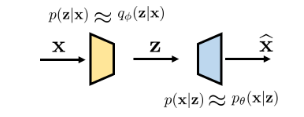
\includegraphics[width=0.5\textwidth]{./pics/VAE.png} % 图片路径和大小
    \caption{VAE block}
\end{figure}
where $q_{\phi}(\mathbf{z} \mid \mathbf{x})$ is the proxy for  $p(\mathbf{z} \mid \mathbf{x})$, which is also the distribution associated with the encoder.  
And $p_{\boldsymbol{\theta}}(\mathbf{x} \mid \mathbf{z})$ is the proxy for  $p(\mathbf{x} \mid \mathbf{z})$ , which is also the distribution associated with the decoder. 
Like the encoder, the decoder can be parameterized by a deep neural network. 

If we treat $\phi$ and $\theta$ as optimization variables, then we need an objective function (or the loss function) so that we can optimize $\phi$ and $\theta$ through training samples.
\begin{definition}[Evidence Lower Bound]
    The Evidence Lower Bound (ELBO) is defined as:
    \begin{equation}
        \operatorname{ELBO}(x) = \mathbf{E}_{q_\phi(z|x)}\left[\log \frac{p(x, z)}{q_\phi(z|x)}\right]
    \end{equation}
\end{definition}
\begin{remark}
    The ELBO is a lower bound of the log-likelihood of the data. It is used to estimate $\log p(x)$.
    \begin{equation}
        \begin{aligned}
            \log p(x) &= \log \int p(x, z) dz\\
            & = \log \int \frac{p(x, z)}{q_\phi(z|x)} \cdot q_\phi(z|x) dz\\
            & \geq \mathbf{E}_{q_\phi(z|x)}\left[\log \frac{p(x, z)}{q_\phi(z|x)}\right] = \operatorname{ELBO}(x)
        \end{aligned}
    \end{equation}
\end{remark}
\begin{theorem}[Decomposition of Log-likelihood]
    We have 
    \begin{equation}
        \log p(x) =\operatorname{ELBO}(x) + \operatorname{KL}(q_\phi(z|x)||p(z|x))
    \end{equation}
    then we can minimize the gap between $\log p(x)$ and ELBO, and the equality hold if and only if $q_\phi(z|x)=p(z|x)$.

    Since $p(z|x)$ is a delta function, 
\end{theorem}
\begin{proof}
    \begin{equation}
        \begin{aligned}
            \log p(x) & = \log p(x)\int q_\phi(z|x)dz\\
            &=\mathbf{E}_{q_\phi(z|x)}\left[\log p(x)\right]\\
            & = \mathbf{E}_{q_\phi(z|x)}\left[\log \left(\frac{p(x, z)}{p(z|x)}\frac{q_\phi(z|x)}{q_\phi(z|x)}\right)\right]\\
            & =\operatorname{ELBO}(x) + \operatorname{KL}(q_\phi(z|x)||p(z|x))
        \end{aligned}
    \end{equation}
\end{proof}

\begin{theorem}
    Also, we can rewrite the ELBO as:
    \begin{equation}
        \begin{aligned}
            \operatorname{ELBO}(x) &= \mathbf{E}_{q_\phi(z|x)}\left[\log p(x|z)+\log p(z)-\log q_\phi(z|x)\right]\\
            &= \mathbf{E}_{q_\phi(z|x)}\left[\log p(x|z)\right] - \operatorname{KL}(q_\phi(z|x)||p(z))\\
            &= \mathbf{E}_{q_\phi(z|x)}\left[\log p_\theta(x|z)\right] - \operatorname{KL}(q_\phi(z|x)||p(z))
        \end{aligned}
    \end{equation}
    where the first term determines how good the decoder is, maxmizing the likelihood of observing the image, 
    and the letter describes how good the encoder is, minimizing the distance between two distributions.
\end{theorem}

\begin{definition}[The objective of VAE]
    The optimiztion objective of VAE is to maxmize the ELBO:
    \begin{equation}
        (\phi, \theta) = \operatorname{argmax}_{\phi, \theta} \sum_{x\in X} \operatorname{ELBO(x)}
    \end{equation}
    where $X$ is the training set.
\end{definition}
\subsection{Diffusion Model}
\paragraph{DDPM}
DDPM is like splitting the encoder and decoder of VAE into controllable parts. 
For each training data point $x_0\sim p_{data}$, then a discrete Markov chain $\{x_1, \cdots, x_N\}$ is constructed by transition function:
\begin{equation}
    p(x_i|x_{i-1})=\mathcal{N}(x_i|\sqrt{1-\beta_i}x_{i-1}, \beta_i I)
\end{equation}
Then we can get 
\begin{equation}
    p_{\alpha_i}(x_i|x_0) = \mathcal{N}(x_i|\sqrt{\alpha_i}x_0, (1-\alpha_i)I), \alpha_i = \Pi_{j=1}^i(1-\beta_j)
\end{equation}
Hence we need to train the ELBO:
\begin{equation}
    \operatorname{ELBO}(x) = \sum_{i=1}^N(1-\alpha_i)\mathbf{E}_{p_{data}(x)}\left[\mathbf{E}_{p_{\alpha_i}(\hat{x}|x)}\left[\|s_\theta(\hat{x}, i) - \nabla_{\hat{x}}\log p_{\alpha_i}(\hat{x}|x)\|\right]\right]
\end{equation}
Then do the reverse Markov chain.

This is clearly a discrete version. Then we consider the continuous version.
We consider linear SDE having the form:
\begin{equation}
    dX_t = (a(t)X_t + b(t))dt + g(t)dW_t
\end{equation}
where $X_t\in \mathcal{R}^d, W_t\in \mathcal{R}^m$ with diffusion factor $Q\in \mathcal{R}^{m\times m}$, then $a(t)\in \mathcal{R}^{d\times d}, b(t)\in \mathcal{R}^d, g(t)\in \mathcal{R}^{d\times m}$. 
By Euler Maruyama method, it can be approximated By
\begin{equation}
    \begin{aligned}
        X_{t+s}&=X_t + (a(t)X_t + b(t))s+g(t)\sqrt{sQ}\xi\\
        &=(1+a(t)s)X_t + b(t)s + g(t)\sqrt{sQ}\xi
    \end{aligned}
\end{equation}
where $\xi\sim N(0, I_m)$. Usually we need to consider the expectation, variance and distribution of $X_t$. But the stochastic value of $X_t$ is dependent of $x_0$. Then first we consider
\begin{equation}
    \begin{aligned}
    E\left[X_{t+s} | X_{0}\right]-E\left[X_{t} | X_{0}\right] & \approx\left(a(t) E\left[X_{t} | X_{t}\right]+b(t)\right) s+g(t) \sqrt{sQ} E[\xi] \\
    & =\left(a(t) E\left[X_{t} | X_{0}\right]+b(t)\right) s .
    \end{aligned}
\end{equation}


Note  $e(t)=E\left[X_{t} | X_{0}\right]$, then
\begin{equation}
    e^{\prime}(t)=\lim _{s \rightarrow 0} \frac{E\left[X_{t+s} | X_{0}\right]-E\left[X_{t} | X_{0}\right]}{s}=a(t) \cdot e(t)+b(t) . \quad e(0)=X_{0} .    
\end{equation}
which is an ODE system, having solution
\begin{equation}
    e(t)=e^{\int_{0}^{t} a(s) d s}\cdot\left(X_{0}+\int_{0}^{t} e^{-\int_{0}^{s} a(r) d r} b(s) d s\right)
\end{equation}
Therefore
\begin{equation}
    \begin{aligned}
    E\left[X_{t}\right] & =E\left[E\left[X_{t} | X_{0}\right]\right]=E[e(t)] \\
    & =e^{\int_{0}^{t} a(s) d s}\cdot\left(E\left[X_{0}\right]+\int_{0}^{t} e^{-\int_{0}^{s} a(r) d r} b(s) d s\right) 
    \end{aligned}
\end{equation}

Similarly, Note $\operatorname{Var}\left(X_{0} | X_{0}\right)=v(t)$:
then $\operatorname{Var}\left(X_{t+s} | X_{0}\right)=(1+s a(t))^{2} \operatorname{Var}\left(X_{t} | X_{0}\right)+s gQg^\top$. Then
\begin{equation}
    \begin{aligned}
        V^{\prime}(t)&=\lim _{s \rightarrow 0} \frac{\operatorname{Var}\left(X_{t+s} | X_{0}\right)-\operatorname{Var}\left(X_{t} | X_{0}\right)}{s}\\
        =&\left[\left(a^{2}(t) s+2 a(t)\right) v(t)+g^{2}(t)\right]|_{s \rightarrow 0}\\ 
        =&2 \alpha(t) V(t)+g(t)Qg^\top(t), \qquad V(0)=0
    \end{aligned}
\end{equation}
Solution is:
\begin{equation}
    v(t)=e^{\int_{0}^{t} 2a(s) d s}\cdot\left(\int_{0}^{t} e^{-\int_{0}^{s} 2 a(r) d r} g(s)Qg^\top(s) d s\right)
\end{equation} 
By law of total variance:
\begin{equation}
    \begin{aligned}
        \operatorname{Var}\left(X_{t}\right)=&E\left[X_{t}^{2}\right]-E^{2}\left[X_{t}\right]=E\left[ E\left[X_{t}^{2} | X_{0}\right]\right]-E^{2}\left[X_{t}\right] \\
        =&E\left[\operatorname{Var}\left(X_{t} | X_{0}\right)+E^{2}\left[X_{t} | X_{0}\right]\right]-E^{2}\left[X_{t}\right] \\
        =&E\left[\operatorname{Var}\left(X_{t} | X_{0}\right)\right]+E\left[E^{2}\left[X_{t} | X_0\right]\right]-E^{2}\left[E\left[X_{t} | X_{0}\right]\right]\\
        =&E\left[\operatorname{Var}\left(X_{t} | X_{0}\right)\right]+\operatorname{Var}\left(E\left[X_{t} | X_0\right]\right)
    \end{aligned}
\end{equation}
then 
\begin{equation}
    \begin{aligned}
        \operatorname{Var}(X_t)=&E[V(t)]+\operatorname{Var}(e(t))\\
        =&e^{\int_{0}^{t} 2 a(s) d s}\cdot \left(\int_{0}^{t} e^{-\int_{0}^{s} 2 a(r) d r} g(s)Qg^\top(s) d s\right) +e^{\int_{0}^{t} 2 a(s) d s} \cdot \operatorname{Var}\left(X_{0}\right) .
    \end{aligned}
\end{equation}

We have the following theorem which is crucial for diffusion models. Usually, we assume $Q=I_m$.
\begin{theorem}
    If  $X_{t+s}=(1+a(t) s) X_{t}+b(t) s+g(t) \sqrt{s} \xi$\\
    then $X_{t} | X_{0} \sim N\left(E\left[X_{t} | X_{0}\right], \operatorname{Var}\left(X_{t} | X_{0}\right)\right)$, 
    where $E\left[X_{t} | X_{0}\right]=e(t), \operatorname{Var}\left(X_{t} | X_{0}\right)=V(t)$.\label{thm1}        
\end{theorem}

It should be noted that $e(t)$ is related to $X_0$ and t, while $V(t)$ only depends on $t$!

Next, we will see how the above formula can be applied to diffusion modtels. There are three frameworks to build SDEs for diffusion models, VP, VE and sub-VP.
\begin{definition}
    Noise function  $\beta(t)$ . s.t. $\beta(0)=0 ; \beta^{\prime}(t) \geqslant 0 ; \beta(t) \rightarrow \infty \text { as } t \rightarrow \infty$
\end{definition}

\textbf{Variance Preserving (VP) SDE}
So if we have diffusion model like:
\begin{equation}
\begin{aligned}
    X_{t_{i+1}}&=\sqrt{1-\left(\beta\left(t_{i+1}\right)-\beta\left(t_{i}\right)\right)}X_{t_i}+\sqrt{\left(\beta\left(t_{i+1}\right)-\beta\left(t_{i}\right)\right)}\xi\\
    &=\sqrt{1-\Delta\beta(t_i)}X_{t_i}+\sqrt{\Delta \beta(t_i)}\xi
\end{aligned}
\end{equation}
Then the conditional distribution is given by:
\begin{equation}
    q\left(X_{t_{i+1}} | X_{t_{i}}\right)=N(x_{t_{i+1}} ; \sqrt{1-\Delta \beta\left(t_{i}\right)}X_{t_i}, \Delta \beta\left(t_{i}\right))
\end{equation}
Then we need to estimate  $\theta$  drift term  $f$  and diffusion term  $g$:

\begin{equation}
    \begin{aligned}
        f(x, t)&=\lim _{h \rightarrow 0} \frac{E\left[X_{t+h}-X_{t} | X_{t}=x\right]}{h} \\
            &=\lim _{h \rightarrow 0} \frac{x \sqrt{1-\Delta \beta(t)}-x}{h}=-\frac{x}{2} \beta^{\prime}(t) . \\
    g(t) &= \sqrt{\lim _{h \rightarrow 0} \frac{N\left[X_{t+h} | X_{t}=x\right]}{h}}=\sqrt{\lim _{h \rightarrow 0} \frac{\beta(t+h)-\beta(t)}{h}}=\sqrt{\beta^{\prime}(t)}
    \end{aligned}
\end{equation}
Then the model can be written as
$d x=-\frac{x}{2} \beta^{\prime}(t) d t+\sqrt{\beta^{\prime}(t)} d W_{t}$


Then we have
\begin{equation}
    \left\{\begin{aligned}
    &E\left[X_{t} | X_{0}\right]=X_{0} e^{\int_{0}^{t}-\frac{1}{2} \beta'(s) d s}=X_{0} e^{-\frac{1}{2} \beta(t)} \\
    &E\left[X_{t}\right]=E\left[X_{0}\right] e^{-\frac{1}{2} \beta(t)} \\
    &V\left(X_{t} | X_{0}\right)=\int_{0}^{t} e^{\int_{0}^{s} \beta^{\prime}(r) d r} \beta^{\prime}(s) d s \cdot e^{-\beta(t)}=1-e^{-\beta(t)} \\
    &V\left(X_{t}\right)=1-e^{-\beta(t)}+V\left(X_{0}\right) e^{-\beta(t)}=1+\left(V\left(X_{0}\right)-1\right) e^{-\beta(t)} .
    \end{aligned}\right.
\end{equation}
So as  $t \rightarrow \infty,\beta(t) \rightarrow \infty$, then  $E \rightarrow 0, V \rightarrow 1$, i.e. 
$X_{t} | X_{0} \sim N\left(E\left[X_{t} | X_{0}\right], \operatorname{Var}\left|X_{t}\right| X_{0}\right)\rightarrow N(0,1) \text{ as } t \rightarrow \infty$.
 
\textbf{Variance-Exploding SDE}
Here is the model: 
$X_{t+h}=X_{t}+\sqrt{\Delta \beta(t)} \xi$

Similarly we can compute the $f(x, t)\equiv 0$ and $g(t)=\sqrt{\beta(t)}$.
Hence  
\begin{equation}\left\{
    \begin{aligned}
        &E\left[X_{0} | X_{0}\right]=X_{0}\\
        &E\left[X_{t}\right]=E\left[X_{0}\right] \\ 
        &V\left(X_{t} | X_{0}\right)=\int_{0}^{t} e^{\int_{0}^{s} 0 d r} \beta^{\prime}(s) d s=\beta(t)\\ 
        &V\left(X_{t}\right)=V\left[X_{0}\right]+\beta(t)
    \end{aligned}\right.
\end{equation}

So the expectation value is constant and the variance is increasing monotonical. \\
If we rescale  $X_{t}$ as $Y_{t}=\frac{X_{t}}{\sqrt{\beta(t)}}$, then $Y_t \rightarrow N(0,1), t \rightarrow \infty$.

\textbf{Sub-VP SDE}
Here, we set the dift and diffusion term as
\begin{equation}
\begin{aligned}
        &f(x, t)=-\frac{1}{2} \beta^{\prime}(t) \\
        &g(t)=\sqrt{\beta^{\prime}(t)\left(1-e^{-2 \beta(t)}\right)}
\end{aligned}
\end{equation}
As the same, we can compute that.
\begin{equation}
    \left\{\begin{aligned}
    &E\left[X_{t} | X_{0}\right]=X_{0} e^{-\frac{1}{2} \beta(t)} \\
    &E\left[X_{t}\right]=E\left[X_{0}\right] e^{-\frac{1}{2} \beta(t)} \\
    &V\left(X_{t} | X_{0}\right)=\left(1-e^{-\beta(t)}\right)^{2} \\
    &V\left(X_{t}\right)=\left(1-e^{-\beta(t)}\right)^{2}+V\left(X_{t}\right) e^{-\beta(t)} .
    \end{aligned}\right.
\end{equation}

We can find out that the variance is always smaller that of VP SDE.

\begin{remark}
    To sum up, finally we hope that $X_t$ converges to a normal distribution by choosing different drift and diffusion functions. 
    For generative model, the goal is to sample from a Data distribution $p_{data}$. We have known that if we set the initial distribution $p_0(x_0)=p(X_0=x_0)\sim p_{data}$, 
    then after $t=T$, the distribution of $X_t$ is tend to be $N(0, 1)$ under certain conditions. 
    
    So the idea is backward: if we sample from $X_T\sim N(0, 1)$, and then run SDE backwards, could we get the initial distribution?
\end{remark}

Assume we have forward SDE: from $X_0\sim p_0,X_T\sim p_T$,
\begin{equation}\label{forward}
    dX_t = f(X_t, t)dt + G(t)dW_t
\end{equation}
Then we define the reverse SDE as: from $X_T\sim p_T$,
\begin{equation}
    d\bar{X_t}=\bar{f}(\bar{X}_t, t)dt + \bar{G}(t)d\bar{W_t}
\end{equation}
where $\bar{W}_t$ is Brownian Motion runns backward in time, i.e. $\bar{W}_{t-s}-\bar{W}_t$ is independent of $\bar{W}_t$. We can approximate by EM:
\begin{equation}
    \bar{X}_{t-s}-\bar{X}_t=-s\bar{f}(\bar{X}_t, t) + \sqrt{s}\bar{G}(t)\xi
\end{equation}
So the problem is: If given $f,G$, are there $\bar{f},\bar{G}$ s.t. the reverse time diffusion process $\bar{X}_t$ has the same distribution as the forward process $X_t$? Yes!
\begin{theorem}
    The reverse SDE with $\bar{f},\bar{G}$ having the following form has the same distribution as the forward SDE \ref{forward}:
    \begin{equation}\left\{
        \begin{aligned}
            &\bar{f}(x,t)=f(x,t)-GG^T\nabla_x\log p_t(x)\\
            &\bar{G}=G(t)
        \end{aligned}\right.
    \end{equation}
    i.e. 
    \begin{equation}
        d\bar{X}_t = \left[f(\bar{X}_t, t)-GG^T\nabla_x\log p_t(x_t)\right]dt+G(t)d\bar{W}_t
    \end{equation}
\end{theorem}
\begin{proof}
    The proof is skipped.
\end{proof}
This theroem allows us to learn how to generate samples from $p_{data}$.
\begin{algorithm}:\\
Step1. Select $f(x, t)$ and $g(t)$ with affine drift coefficients s.t. $X_T\sim N(0, 1)$\\
Step2. Train a network $s_\theta(x, t)=\frac{\partial}{\partial x}\log p_t(x)$ where $p_t(x)=p(X_t=x)$ is the forward distribution.\\
Step3. Sample $X_T$ from $N(0, 1)$, then run reverse SDE from T to 0:
\begin{equation}
    \bar{X}_{t-s} = \bar{X}_t + s\left[g^2(t)s_\theta(\bar{X}_t, t)-f(\bar{X}_t, t)\right] + \sqrt{s}g(t)\xi
\end{equation}
\end{algorithm}
\begin{figure}[h]
    \centering
    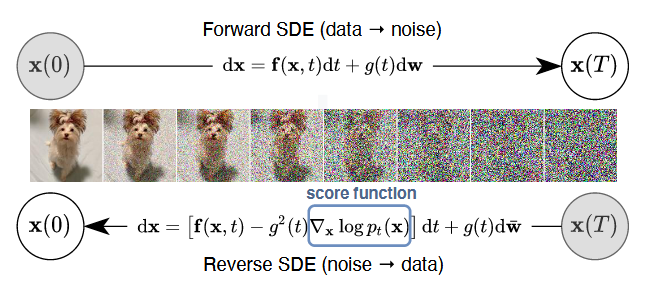
\includegraphics[width=0.8\textwidth]{./pics/score_based.png} % 图片路径和大小
    \caption{score-based generative model}
\end{figure}


\subsection{Score Matching}
The most difficult question on how to obtian $\nabla_x \log p(x)$ because it solves FPK equation.

\textbf{subsubsection}{Explicit Score Matching}
Suppose we have a set of samples $x_1, x_2, \cdots, x_n$ from the data distribution $p_{data}(x)$. 
A classical way is to consider the kernel density estimation $q(x)$ of $p(x)$:
\begin{equation}
    q(x) = \frac{1}{n}\sum_{i=1}^n K(x-x_i)
\end{equation}
where $K(x)$ is the kernel function. Since $q(x)$ is an approximation to $p_{data}$. 
We can define a loss function to train a network:
\begin{equation}
    \begin{aligned}
        \mathcal{L}_\theta =& \mathbf{E}_{x\sim p(x)} \left[\left\|s_\theta(x) - \nabla_x \log p(x)\right\|^2\right]\\
        \approx& \mathbf{E}_{x\sim q(x)} \left[\left\|s_\theta(x) - \nabla_x \log q(x)\right\|^2\right]\\
        =& \int \left\|s_\theta (x) - \nabla_x \log q(x)\right\|^2 q(x) dx\\
        \approx & \frac{1}{n}\sum_{i=1}^n \int \left\|s_\theta (x) - \nabla_x \log q(x)\right\|^2 K(x-x_i) dx
    \end{aligned}
\end{equation}
However, when the number of samples is limited, the estimation $\nabla_x \log q(x)$ is not accurate.

\textbf{Implicit Score Matching}

\textbf{Denoising Score Matching}
Normally we can define the loss function as follows:
\begin{equation}
    \begin{aligned}
        L_\theta & = \frac{1}{T}\int_0^T\lambda(t)\underset{x_0\sim p_{data}}{E}\left[\underset{x_t\sim p_{t|0}(x_t|x_0)}{E}\left[\|s_\theta(x_t, t)-\nabla_{x_t}\log p_t(x_t)\|^2\right]\right]dt\\
        &=\underset{t\sim U(0, T)}{E}\left[\lambda(t)\underset{x_0\sim p_{data}}{E}\left[\underset{x_t\sim p_{t|0}(x_t|x_0)}{E}\left[\|s_\theta(x_t, t)-\nabla_{x_t}\log p_t(x_t)\|^2\right]\right]\right]
    \end{aligned}
\end{equation}
It should be clearified that $p_{t|0}(x_t|x_0)=p(X_t=x_t|X_0=x_0)$. So $$p_t(x_t)=\int p_{t|0}(x_t|x_0)p_0(x_0)dx_0=E_{x_0\sim p_{data}}\left[p_{t|0}(x_t|x_0)\right]$$
where $p_{t}(x)=p\left(X_{t}=x\right)$, $p_{t | 0}(x | y)=p\left(X_{t}=x | X_{0}=y\right)$. Then

\begin{equation}
    \begin{aligned}
    \nabla \log p_{t}(x) & =\frac{1}{p_{t}(x)} \nabla p_{t}(x) . \\
    & =\frac{1}{p_{t}(x)} \nabla \int p_{t | 0}(x | y) p_{0}(y) d y \\
    & =\frac{1}{p_{t}(x)} \int \nabla p_{t | 0}(x | y) p_{0}(y) d y \\
    & =\frac{1}{p_{t}(x)} \int \frac{\nabla p_{t | 0}(x | y)}{p_{t | 0}(x | y)} p_{0}(y) \cdot p_{t | 0}(x | y) d y \\
    & =\int \nabla_{x} \log \left(p_{t | 0}(x | y)\right) \cdot p_{0 | t}(y | x) d y \\
    & =\underset{y\sim p_{0|t}(y|x)}{E}\left[\nabla_{x} \log \left(p_{t | 0}(x | y)\right)\right]
    \end{aligned}
\end{equation}

Where we have used the following lemma:
\begin{lemma}
    \begin{equation}
        \underset{x_0\sim p_0}{E}\left[\underset{x_t\sim p_{t|0}(\cdot|x_0)}{E}\left[\underset{x'_0\sim p_{0|t}(\cdot|x_t)}{E}\left[f(x_t, x'_0)\right]\right]\right]=\underset{x_0\sim p_0}{E}\left[\underset{x_t\sim p_{t|0}(\cdot|x_0)}{E}\left[f(x_t, x_0)\right]\right]
    \end{equation}
\end{lemma}
\begin{proof}
    Easy to prove.
\end{proof}
Then we can rewrite the loss function as:
\begin{equation}
    \begin{aligned}
        L_{\theta}&=\underset{t\sim U(0,T)}{E}\left[\lambda(t) \underset{x_{0}\sim p_{data}}{E}\left[\underset{x_{t}\sim p_{t|0}(x_t|x_0)}{E}\left[\left\|S_{\theta}\left(x_{t}, t\right)-\nabla _{x_t}\log p_{t}\left(x_{t}\right)\right\|^{2}\right]\right.\right.\\ 
        &\leqslant \underset{t\sim U(0,T)}{E}\left[\lambda(t) \underset{x_{0}\sim p_{data}}{E}\left[\underset{x_{t}\sim p_{t|0}(x_t|x_0)}{E}\left[\underset{y\sim p_{data}}{E}\left[\left\|S_{\theta}\left(x_{t}, t\right)-\nabla_{x_{t}} \log \left(p_{t|0}(x_t | y)\right)\right\|^{2}\right]\right]\right]\right] \\
        &=\underset{t\sim U(0, T)}{E}\left[\lambda(t) \underset{x_{0}\sim p_{data}}{E}\left[\underset{x_{t}\sim p_{t|0}(x_t|x_0)}{E}\left[\| S_{\theta}\left(x_{t}, t\right)-\nabla_{x_{t}} \log \left(p_{t|0}\left(x_{t} | x_{0}\right) \|^{2}\right]\right]\right]\right.
    \end{aligned}
\end{equation}


Since  $p_{t|0}\left(x_{t} | x_{0}\right)=p\left(X_{t}=x_{t} | X_{0}=x_{0}\right)$  has been discussed:

$$p_{t | 0}\left(x_{t} | x_{0}\right) \sim N\left(x_{t} ; E\left[X_{t}=x_t | X_{0}=x_{0}\right], \operatorname{Var}\left(X_{t}=x_t | X_{0}=x_{0}\right)\right) .$$

Then by theorem \ref{thm1}, x can be written as $x=e(t, X_0)+\sqrt{V(t)}\xi$, where $\xi\sim N(0, 1)$, then the score function is:
\begin{equation}
    \frac{\partial}{\partial x} \log p_{t | 0}\left(x | x_{0}\right)=-\frac{x-E_{t | 0}\left[x | x_{0}\right]}{\operatorname{Var}_{t | 0}\left(x | x_{0}\right)}=-\frac{x-e(t, X_0)}{V(t)}\sim -N\left(0, \frac{1}{V(t)}\right)
\end{equation}
So
\begin{equation}
\begin{aligned}
    L_\theta=&\underset{t\sim U(0,T)}{E}\left[\lambda (t)\underset{x_0\sim p_{data}}{E}\left[\underset{\xi\sim N(0, 1)}{E}\left[\left\|s_\theta\left(\sqrt{V(t)}\xi+e(t, X_0), t\right) + \frac{\xi}{\sqrt{V(t)}}\right\|^2\right]\right]\right]\\
    =&\underset{t\sim U(0,T)}{E}\left[\lambda (t)\underset{x_0\sim p_{data}}{E}\left[\frac{1}{V(t)}\underset{\xi\sim N(0, 1)}{E}\left[\left\|\xi_\theta\left(\sqrt{V(t)}\xi+e(t, X_0), t\right)-\xi\right\|^2\right]\right]\right]
\end{aligned}    
\end{equation}
where $\xi_\theta = -\sqrt{V(t)}s_\theta$ is called denoising network.

\subsection{Denoising Diffusion}

\subsubsection{With Classifier Guidance}
Though we can produce pictures by sampling from normal distribution, we still cannot control what we will generate. What we want to do is something like:
"Give me the pictures of number 6", then the model can sample from the normal distribution and do the denoising to generate pics of 6. 

Usually, we can do something like: train a model for every class label. This do make the model smaller, but increases number of models. 
Think about it, when the label is TEXT, it is impossiable to train a model for each sentences. 

So, the initial distribution is $p_0(x|y)$ given the label y. Similarly, we will convert the data distribution $p_{data}(x|y)$ to final distribution, normal distribution expected.
Then we SDE becomes: $X_t \sim p_t(x|y)$


\begin{equation}
    \begin{aligned}
    & p_{t}(x \mid y)=p\left(X_{t}=x \mid y\right)=\frac{p\left(y \mid X_{t}=x\right) p\left(X_{t}=x\right)}{p(y)} \\
    \Rightarrow & \log \left(p_{t}(x \mid y)\right)=\log \left(p\left(y \mid X_{t}=x\right)\right)+\log \left(p\left(X_{t}=x\right)\right)-\log (p(y)) \\
    \Rightarrow & \nabla_{x} \log \left(p_{t}(x \mid y)\right)=\nabla_{x} \log \left(p\left(y \mid X_{t}=x\right)\right)+\nabla_{x} \log \left(p\left(X_{t}=x\right)\right)
    \end{aligned}
\end{equation}
    
    
We have finished training  $\nabla_{x} \log \left(p\left(X_{t}=x\right)\right)$  in sampling. Then we need to estimate  $\nabla_{x} \log \left(p\left(y \mid X_{t}=x\right)\right)$. This is the conditional protability, we end up with a sharp factor s: $p^{\prime}\left(y \mid X_{t}=x\right)$ , then:
\begin{equation}
    \nabla_{x} \log \left(p_{t}(x \mid y)\right)=S \nabla_{x} \log \left(p\left(y \mid x_{t}=x\right)\right)+\nabla_{x} \log \left(p\left(x_{t}=x\right)\right)
\end{equation}
Note  $\omega_{\theta}(y \mid x, t)$  to learn  $s \nabla_{x} \log \left(p\left(y \mid X_{t}=x\right)\right)$ 

\subsubsection{Classifier Guidance Free}
\begin{equation}
    \begin{aligned}
        &\gamma \nabla_{x} \log \left(p\left(y \mid X_{t}=x\right)\right)\\
         =& \gamma\left(\nabla_x \log \left(p(X_t=x|y)\right) - \nabla_x \log \left(p_t(x)\right)\right)
    \end{aligned}
\end{equation}
Then 
\begin{equation}
    \begin{aligned}
        &\nabla_{x} \log_\gamma \left(p_{t}(x \mid y)\right)\\
        =&(1-\gamma)\nabla_x \log \left(p_t(x)\right) + \gamma\nabla_x \log \left(p(X_t=x|y)\right)
    \end{aligned}
\end{equation}
Hence we only need one conditional denoising network, and using null condition to represent the unconditional model.

\subsection{Flow Matching}
We have discussed the FPK Equation in 'learnsde'. 
\begin{theorem}[Fokken-Planck-Kolmogorov equation]
    The density function $p(x, t)$ of $X_t$ s.t. 
    \begin{equation}
        dX_t = f(X_t, t)dt + G(X_t,t)dW_t
    \end{equation}
    solves the PDE:
    \begin{equation}
        \frac{\partial p(x, t)}{\partial t}=-\sum_{i} \frac{\partial}{\partial x_{i}}\left[f_{i}(x, t) p(x, t)\right]+\frac{1}{2} \sum_{i, j} \frac{\partial^{2}}{\partial x_{i} \partial x_{j}}\left[\left(G Q G^{\top}\right)_{i j} p(x, t)\right]
    \end{equation}
    The PDE is called FPK equation / forwand Kolmogorov equation.
\end{theorem}
It can be rewritten as:
\begin{equation}
    \begin{aligned}
        \frac{\partial p(x, t)}{\partial t} &= -\nabla\cdot\left[f(x, t) p(x, t)\right]+\frac{1}{2} \nabla^2\cdot\left[\left(G Q G^{\top}\right) p(x, t)\right] \\
        &=-\nabla\cdot\left[f(x, t) p(x, t)-\frac{1}{2} \nabla\cdot\left[\left(G Q G^{\top}\right) p(x, t)\right]\right]
    \end{aligned}
\end{equation}
Here, if we only consider $G(X_t, t)=g(t)$, then we notice that $M=GQG^T$ is independent of $X_t$, so we can write:
\begin{equation}
    \begin{aligned}
        \frac{\partial p(x, t)}{\partial t} &= -\nabla\cdot\left(fp-\frac{1}{2}\nabla\cdot (Mp)\right)\\
        &=-\nabla\cdot\left(fp-\frac{1}{2}M\nabla p\right)\\
        &=-\nabla\cdot\left[\left(f-\frac{1}{2}M\frac{\nabla p}{p}\right)p\right]\\
        &=-\nabla\cdot\left[\left(f-\frac{1}{2}M\nabla\log p\right)p\right]
    \end{aligned}
\end{equation}
So we find out that if we have an ODE s.t. $dZ_t=F(Z_t, t)dt$ with $Z_0 \sim p_0$, instead of a SDE, then by FPK equation, the density $p(z, t)$ satisfies:
\begin{equation}
    \frac{\partial p(z, t)}{\partial t}=-\nabla\cdot\left(F(z, t)p(z, t)\right)
\end{equation}
So if we set $F(z, t)=f(z, t) - \frac{1}{2}M(t)\nabla\log p(z, t)$, then $p(z, t)$ is exactly like the density $p(x, t)$ of $X_t$ in SDE. 
So theoretically, we can do the diffusion like reverse ode!

This is the topic discussed in 'Probability Flow'.

Define a flow $\phi: \mathcal{R}^d\times [0, 1]\rightarrow \mathcal{R}^d$ is a flow generated by a vector field $v: \mathcal{R}^d \times [0, 1]\rightarrow \mathcal{R}^d$ i.e.
\begin{equation}\left\{
    \begin{aligned}
        \frac{\partial \phi(x, t)}{\partial t} &= v(\phi(x, t), t)\\
        \phi(0, x)&=x
    \end{aligned}\right.
\end{equation}
The flow means that under the vector field $v$, if the initial point is $x$, then the flow push the point after time $t$ to $\phi(x, t)$. That is $\phi$ gives the evolution trajectory of $x$ under the vector field $v$.
So normally, we can consider the flow $\phi(x, t)$ as $X_t$ in SDE:
\begin{equation}
    dX_t = v(X_t, t)dt + 0dW_t
\end{equation}
with $X_0=x$. It turns out that it is actually an ODE, a SDE without diffusion term. Similar to SDE, if $X_0=x\sim p_0(x)$, we have the probability density $p(x, t)$ satisfies FPK equation:
\begin{equation}
    \frac{\partial p(x, t)}{\partial t}=-\nabla\cdot\left(v(x, t)p(x, t)\right)
\end{equation}
which is a special case of FPK equation, called \textbf{Continuity Equation}. So, typically, we can solution to an ODE is a flow.



So the objective of Flow Matching Model can be described as: Let $p_t(x)$ be the density with initial $p_0(x)$, which is designed to be a simple distribution, like normal distribution. 
So let $p_1(x)$ be the approximation equal in distribution to$ p_{data}$. Then we need to design a flow to match the flow s.t. $p_1$ can properly approximate $p_{data}$.

\section{Random Field}
\subsection{Definitions}
\begin{definition}[Random Field]
    For a set $D\subset \mathbb{R}^d$, a (real-valued) random field ${u(x):x\in D}$ is a set of real-valued 
    random variables on a probability space $(\Omega, \mathcal{F}, P)$. We usually speak of realizations of random field, instead of sample paths. 
\end{definition}

\begin{definition}[second-order random field]
    A random field is called second-order random field if $u(x)\in L^2(\Omega)$ for $\forall x\in D$. With its mean and covariance function:
    \begin{equation}\left\{
        \begin{aligned}
            \mu(x) &= \mathbf{E}[u(x)]\\
            C(x, y) &= Cov(u(x), u(y))=\mathbf{E}[(u(x)-m(x))(u(y)-m(y))]\\
        \end{aligned}\right.
    \end{equation}
\end{definition}

\begin{definition}[Gaussian Random Field]
    A second-order random field ${u(x):x\in D}$ is called Gaussian random field if 
    \begin{equation}
        u = u[u(x_1), u(x_2), \cdots, u(x_n)]^T \sim \mathcal{N}(\mu(x), C(x, y)),\ \forall x_i \in D
    \end{equation}
\end{definition}

\begin{example}[$L^2(D)$-valued random variable]
    For $D\subset \mathbb{R}^d$, consider $L^2(D)$-valued R.V. u with $\mu \in L^2(D)$ and $\mathscr{C}$.
    Then $u(x)$ is a real-valued random field for each $x\in D$, and mean and covariance are well defined.

    Meanwhile, for $\phi, \psi \in L^2(D)$, we have
    \begin{equation}
        \begin{aligned}
            \langle \mathscr{C}\phi, \psi \rangle &= Cov\left(\langle u, \phi \rangle_{L^2(D)}, \langle u, \psi \rangle_{L^2(D)}\right)\\
            &=E\left[\left(\int_D \phi(x)(u(x)-\mu(x))dx\right)\left(\int_D \psi(y)(u(y)-\mu(y))dy\right)\right]\\
            &=\int_D \int_D \phi(x)\psi(y)E[(u(x)-mu(x))(u(y)-mu(y))]dxdy\\
            &=\int_D \int_D \phi(x)\psi(y)Cov(u(x), u(y))dxdy\\
        \end{aligned}
    \end{equation}
    So that
    \begin{equation}
        (\mathscr{C}\phi)(x) = \int_D Cov(u(x), u(y))\phi(y)dy
    \end{equation}
    which is the covariance function of the random field $u(x)$. So, any $L^2(D)$-valued random variable defines a second-order random field, 
    with mean $\mu(x)$ and covariance $C(x, y) = Cov(u(x), u(y))$ which is the kernel of the covariance operator $\mathscr{C}$.
\end{example}

\begin{example}[Stationary Random Field]
    A second-order random field ${u(x): x\in D}$ is called stationary if the mean is constant and covariance function 
    depends only on the difference $x-y$, i.e. $\mu(x) = \mu,\ C(x, y) = C(x-y)$.
\end{example}

\begin{theorem}[Wiener-Khinchin Theorem]
    There exists a stationary random field ${u(x): x\in D}$ with mean $\mu$ and covariance function $c(x)$ that is mean square continuous if and only if 
    the function $c(x): \mathbb{R}^d\rightarrow \mathbb{R}$ is such that 
    \begin{equation}
        c(x) = \int_{\mathbb{R}^d} e^{iv \cdot x}dF(v) = (2\pi)^{\frac{d}{2}}\hat{f}(x)
    \end{equation}
    where $F(v)$ is some measure on $\mathbb{R}^d$ and $\hat{f}(x)$ is the Fourier transform of $f(x)$, f is the density function of $F$.
    
    Reversely, $f(v) = (2\pi)^{\frac{d}{2}}\hat{c}(v)$.
    If $f$ is non-negative and integrable, then $c(x)$ is a valid covariance function.
\end{theorem}

\begin{example}[Isotropic Random Field]
    A stationary random field is called isotropic if its covariance function depends only on the distance between points, i.e.
    \begin{equation}
        Cov(x) = c(\|x\|_2) = c^0(r)
    \end{equation}
    where $c^0$ is known as the isotropic covariance function.
\end{example}
\subsection{Algorithms}
In 2D cases, the covariance matrices of samples of stationary random fields $u(x)$ at uniformly spaced points $x\in D$ are symmetric BTTB matrices.
\begin{definition}[Uniformly spaced points]
    Let $D = [0,a_1]\times[0,a_2]$, the uniformly spaced points are given by:
    \begin{equation}
        x_k = x_{i,j} = (i\Delta x_1, j\Delta x_2)^T,\ i = 0, 1, \cdots, n_1-1,\ j = 0, 1, \cdots, n_2-1, k=i+j n_1
    \end{equation}
    where $\Delta x_1 = \frac{a_1}{n_1-1}$ and $\Delta x_2 = \frac{a_2}{n_2-1}$. 
    
    With $N=n_1n_2$, $u = [u_0, u_1, \cdots, u_{N-1}]^T\sim \mathcal{N}(0, C)$ is the vector of samples of $u(x)$ at the uniformly spaced points.
    Since $u(x)$ is stationary, $C$ is a $N\times N$ symmetric BTTB matrix with elements:
    \begin{equation}
        C_{kl} = Cov(u_k, u_l) = c(x_{{i+jn_1}} - x_{r+sn_1})
    \end{equation}
    where $c(x_k - x_l)$ is the covariance function of $u(x)$. 
\end{definition}


\begin{theorem}
    The covariance matrix $C$ is always a symmetric BTTB matrix.
\end{theorem}

Since we have the Fourier representation of BCCB matrix and BTTB matrix can by extended to BCCB by even extension, we can use the following algorithm to generate the samples of $u(x)$.
So, when the even BCCB extension $\tilde{C}\in \mathbb{R}^{4N\times 4N}$ is non-negative definite, then $N(0, \tilde{C})$ is a valid Gaussian distribution.

\begin{algorithm}
    Suppose the even BCCB extension $\tilde{C}\in \mathbb{R}^{4N\times 4N}$ is non-negative definite, and the leading principle submatrix $S\in \mathbb{R}^{2N\times 2N}$ is:
    \begin{equation}
        S = \begin{pmatrix}
            \tilde{C}_0 & \tilde{C}_1^T & \cdots & \tilde{C}_{n_2-1}^T\\
            \tilde{C}_1 & \tilde{C}_2 & \cdots & \tilde{C}_{n_2-2}^T\\
            \vdots & \vdots & \ddots & \vdots\\
            \tilde{C}_{n_2-1} & \tilde{C}_{n_2-2} & \cdots & \tilde{C}_0
        \end{pmatrix},\quad \tilde{C}_i = \begin{pmatrix}
            C_i & B_i\\
            B_i & C_i
        \end{pmatrix}
    \end{equation}
    where $C_i, B_i \in \mathbb{R}^{n_1\times n_1}$, $i = 0, 1, \cdots, n_2-1$. 
    
    Now given $\tilde{u}\sim N(0, \tilde{C})$, let $v$ be the first $2n_1n_2$ elements of $\tilde{u}$, 
    then $v\sim N(0, S)$. Take the first $n_1$ elements of $v$ per $2n_1$ elements to get $\tilde{v}\sim N(0, C)$.
\end{algorithm}

However, when the even BCCB extension $\tilde{C}\in \mathbb{R}^{4N\times 4N}$ is indefinite, we can avoid this by padding. 
But sometimes, padding leads to the size of matrix explosion. Approximate circulant embedding may be the only option.

\subsection{KL expansion of R.F.}
As mentioned before, we have the underlying covariance operator defined by:
\begin{equation}
    (\mathscr{C}\phi)(x) = \int_D Cov(u(x), u(y))\phi(y)dy=\int_D c(x-y)\phi(y)dy
\end{equation}
Hence, for the covariance operator $\mathscr{C}$, we have the eigenfunctions with corresponding eigenvalues $\{v_j, \phi_j\}_{j=1}^{\infty}, v_j\geq v_{j-1}$.
\begin{theorem}[$L^2$ convergence of KL expansion]
    Let $D\subset \mathbb{R}^d$, consider a random field $u(x): x\in D$ and $u\in L^2(\Omega, L^2(D))$, then:
    \begin{equation}
        u(x) = \mu(x) + \sum_{j=0}^{\infty} \sqrt{v_j} \phi_j(x) \xi_j
    \end{equation}
    where the sum converges in $L^2(\Omega, L^2(D))$, 
    \begin{equation}
        \xi_j = \frac{1}{\sqrt{v_j}}\int_D (u(x)-\mu(x))\phi_j(x)dx
    \end{equation}
    The random variables $\xi_j$ have mean zero, unit variance and are pairwise uncorrelated.
    If u is Gaussian, then $\xi_j$ are i.i.d. Gaussian random variables with zero mean and unit variance.
\end{theorem}

\section{Stationary SPDEs}
\subsection{Definition}
\begin{definition}[Stationary SPDE]
    Assume given $a, f\in L^2(\Omega, L^2(D))$ are random fields, try to seek $u:\bar{D}\times \Omega \to \mathbb{R}$ in weak sense s.t. $\mathbb{P}$-a.s.:
    \begin{equation}\left\{
        \begin{aligned}
            -\nabla \cdot (a(x, w)\nabla u(x, w)) = f(x, w),\qquad x\in D\\
            u(x, w) = g(x),\qquad x\in \partial D
        \end{aligned}\right.\label{spde1model}
    \end{equation}
    To ensure the existence of solution, we need to impose some conditions on $g$.
\end{definition}

\begin{definition}[Weak solution on $D\times \Omega$]
    A weak solution to Eq(\ref{spde1model}) with $g=0$ is a function $u\in V=L^2(\Omega, H_0^1(D))$ s.t. for any $v\in V$,
    \begin{equation}
        a(u, v) = l(v)\label{spde1weak}
    \end{equation}
    where\begin{equation}\left\{
        \begin{aligned}
            a(u, v) &= E\left[\int_D a(x, \cdot)\nabla u(x, \cdot)\cdot \nabla v(x, \cdot)dx\right]\\
            l(v) &= E\left[\int_D f(x, \cdot)v(x, \cdot)dx\right]
        \end{aligned}\right.
    \end{equation}
    If $g\neq 0$, a weak solution to Eq(\ref{spde1model}) is a function $u\in W=L^2(\Omega, H_g^1(D))$ s.t. for any $v\in V$,
    \begin{equation}
        a(u, v) = l(v)\label{spde1weaknh}
    \end{equation}
    where $a(\cdot, \cdot):W\times V\to \mathbb{R}$ and $l:V\to \mathbb{R}$:
    \begin{equation}\left\{
        \begin{aligned}
            a(u, v) &= E\left[\int_D a(x, \cdot)\nabla u(x, \cdot)\cdot \nabla v(x, \cdot)dx\right]\\
            l(v) &= E\left[\int_D f(x, \cdot)v(x, \cdot)dx\right]
        \end{aligned}\right.
    \end{equation}
\end{definition}

\begin{theorem}[Existence and uniqueness of weak solution]
    Note for all $x\in D$
    \begin{equation}\label{assumption1}
        0<a_{\min}\leq a(x, \cdot)\leq a_{\max}<\infty
    \end{equation} as a basic assumption.

    If $f\in L^2(\Omega, L^2(D)),g=0$, and Assumption (\ref{assumption1}) holds, then SPDE \ref{spde1weak} has a unique weak solution $u\in V$.

    If Assumption (\ref{assumption1}) holds, $f\in L^2(\Omega, L^2(D))$, and $g\in H^{\frac{1}{2}}(\partial D)$, 
    then SPDE \ref{spde1weaknh} has a unique weak solution $u\in W$.
\end{theorem}

Assume we have the approximate random fields $\tilde{a}, \tilde{f}: D\times \Omega \to \mathbb{R}$ s.t. (\ref{assumption1}) holds.

Then as mentioned before, we can expand $a, f$ in terms of (truncated) Karhunen-Loeve expansion as:
\begin{equation}\left\{
    \begin{aligned}
        &a(x, w) = \mu_a(x) + \sum_{i=1}^{N_a}\sqrt{v_i^a}\phi_i^a(x)\xi_i^a(w)\\
        &f(x, w) = \mu_f(x) + \sum_{i=1}^{N_f}\sqrt{v_i^f}\phi_i^f(x)\xi_i^f(w)
    \end{aligned}\right.\label{expansion}
\end{equation}
where $(v_i^a, \phi_i^a), (v_i^f, \phi_i^f)$ are the eigenpairs of the covariance operators of $a, f$ respectively, 
and $\xi_i^a, \xi_i^f$ are i.i.d. random variables.

The next question is how to compute:
\begin{equation}
    \begin{aligned}
        a(u, v) &= E\left[\int_D a(x, \cdot)\nabla u(x, \cdot)\cdot \nabla v(x, \cdot)dx\right]\\
        &=\int_\Omega \int_D a(x, w)\nabla u(x, w)\cdot \nabla v(x, w)dxdP(w)\\
    \end{aligned}
\end{equation}

Since the truncated KL expansion of $a(x, w)$ depends on a finite number $N_a$ of random variables $\xi_i^a:\Omega\to \Gamma_i$(same as $f(x,w)$), 
we consider weak form of Eq(\ref{spde1model}) on $D\times \Gamma$, where $\Gamma = \prod_{i=1}^{N_a}\Gamma_i$.

\begin{definition}[finite-dimensional noise]
    A function $v\in L^2(\Omega, L^2(D))$ of the form $v(x, \xi(w))$ for $\forall x\in D,w\in \Omega$, where $\xi = [\xi_1, \cdots, \xi_{N}]^T:\Omega\to \Gamma$, is called a finite-dimensional noise.
\end{definition}

\begin{definition}[Weak solution on $D\times \Gamma$]
    Let $\tilde{a}(x)$ and $\tilde{f}(x)$ be finite-dimensional noises defined in Eq(\ref{expansion}), then the solution to Eq (\ref{spde1model}) is also finite-dimensional noise. 
    Define
    \begin{equation}
        W:=L^2_p(\Gamma, H^1_g(D)) = \left\{v:D\times \Gamma\to \mathbb{R}: \int_\Gamma \|v(\xi, \cdot)\|_{H^1_g(D)}^2d\xi<\infty\right\}
    \end{equation}
    A weak solution to Eq(\ref{spde1model}) on $D\times \Gamma$ is a function $u\in W=L^2_p(\Gamma, H^1_g(D))$ s.t. for any $v\in V=L^2_p(\Gamma, H^1_0(D))$,
    \begin{equation}
        a(u, v) = l(v)\label{weakfd}
    \end{equation}
    where
    \begin{equation}\left\{
        \begin{aligned}
            a(u, v) &= \int_\Gamma p(\xi)\int_D \tilde{a}(x, \xi)\nabla u(x, \xi)\cdot \nabla v(x, \xi)dxd\xi\\
            l(v) &= \int_\Gamma p(\xi)\int_D \tilde{f}(x, \xi)v(x, \xi)dxd\xi
        \end{aligned}\right.
    \end{equation}
\end{definition}
\subsection{Stochastic Galerkin Method}
Therefore, we have the stochastic Galerkin solution: seek $u_{hk}\in W^{hk}\subset L^2(\Gamma, H^1_g(D))$ s.t. for any $v_{hk}\in V^{hk}\subset L^2(\Gamma, H^1_0(D))$.

By define the inner product:
\begin{equation}
    \langle v, w\rangle_{p} = \int_\Gamma v(\xi)w(\xi)P(\xi)d\xi
\end{equation}
We can construct a sequence of polynomials $P_i(\xi)$ on $\Gamma$. Hence:
\begin{equation}
    L^2_p(\Gamma):=\{v:\Gamma\to \mathbb{R}: \|v\|^2_{L^2_p(\Gamma)} = \langle v, v\rangle_p<\infty\}
\end{equation}

\begin{definition}
    Note $S^k$ be the set of polynomials of degree $k$ or less on $\Gamma$:
    \begin{equation}
        \begin{aligned}
            S^k &= \operatorname{span}\{\prod_{i=1}^{M}P_i^{\alpha_i}(\xi_i): \alpha_i\in \mathbb{N}_0, \sum_{i=1}^{M}\alpha_i\leq k\}\\
            &= \operatorname{span}\{\psi_1, \psi_2, \cdots, \psi_Q\}
        \end{aligned}
    \end{equation}
    where $P_i(\xi_i)$ is some polynomial. And $Q=\operatorname{dim}S^k = \binom{M+k}{k}$.
\end{definition}
We need $S^k\subset L^2_p(\Gamma)$ where $\Gamma \subset \mathbb{R}^M$. If $\{\xi_i\}$ are independent, then the joint density $p$ is:
\begin{equation}
    p(\xi) = \prod_{i=1}^{M}p_i(\xi_i)
\end{equation}
Recall $V^h=\operatorname{span}\{\phi_i\}_{i=1}^{J}\subset H^1_0(D)$ is the finite element space, we have tensor product space:
\begin{equation}
    V^{hk}:= V^h\otimes S^k = \operatorname{span}\{\phi_i\psi_j\}_{i=1, j=1}^{J,Q}
\end{equation}

Then 
\begin{equation}
    W^{hk}:=V^{hk}\oplus \operatorname{span}\{\phi_{J+1},\cdots, \phi_{J+J_{b}}\}
\end{equation}
where $J_b$ is finite element functions associated with Dirichlet boundary vertices.

\begin{theorem}[Stochastic basis functions]
    If $\{\xi_i\}$ are independent, suppose that $\{P_i^{\alpha_i}(\xi_i)\}_{\alpha_i=1}^{M}$ are orthonormal with $\langle\cdot,\cdot\rangle_{p_i}$ on $\Gamma_i$.
    Then the complete orthonormal polynomials $\{\psi_j\}_{j=1}^{Q}$ are orthonormal with $\langle\cdot,\cdot\rangle_p$ on $\Gamma$.
\end{theorem}

Then $u_{hk}$ can be written as:
\begin{equation}
    u_{hk}(x, \xi) = \sum_{i=1}^{J}\sum_{j=1}^{Q}u_{ij}\phi_i(x)\psi_j(\xi)+w_g
\end{equation}

\begin{theorem}[Mean and covariance]
    The Galerkin solution can be rewritten as:
    \begin{equation}
        \begin{aligned}
            u_{hk}(x, \xi) &=\sum_{i=1}^{J}\left(\sum_{j=1}^{Q}u_{ij}\phi_i(x)\right)\psi_j(\xi)+w_g\\
            &=\sum_{j=1}^{Q}u_j\psi_j(\xi)+w_g\\
            &= (u_1(x)+w_g(x))\psi_1(\xi) + \sum_{j=2}^{Q}u_j(x)\psi_j(\xi)\\
        \end{aligned}
    \end{equation}
    Then the mean and covariance is 
    \begin{equation}\left\{
        \begin{aligned}
            E[u_{hk}] &= u_1+w_g\\
            Var(u_{hk}) &= \sum_{j=2}^{Q}u_j^2
        \end{aligned}\right.
    \end{equation}
\end{theorem}
\subsection{Algorithm}
Expand $u_{hk}$ in terms of basis functions $v = \phi_r \psi_s$ for $r=1,2,\cdots, J, s=1,2,\cdots, Q$, we have the linear system:
\begin{equation}
    A = \begin{pmatrix}
        A_{11} & A_{12} & \cdots & A_{1Q}\\
        A_{21} & A_{22} & \cdots & A_{2Q}\\
        \vdots & \vdots & \ddots & \vdots\\
        A_{Q1} & A_{Q2} & \cdots & A_{QQ}
    \end{pmatrix},
    \mathbf{u} = \begin{pmatrix}
        \mathbf{u}_1\\
        \mathbf{u}_2\\
        \vdots\\
        \mathbf{u}_Q
    \end{pmatrix},
    \mathbf{b} = \begin{pmatrix}
        \mathbf{b}_1\\
        \mathbf{b}_2\\
        \vdots\\
        \mathbf{b}_Q
    \end{pmatrix}
\end{equation}
where
\begin{equation}
    \mathbf{u}_j = [u_{1j}, u_{2j}, \cdots, u_{Jj}]^T, j=1,2,\cdots, Q
\end{equation}
and each submatrix $A_{sj}$ is a $J\times J$ matrix:
\begin{equation}
    A_{sj} = \langle \phi_r, \frac{\partial \psi_s}{\partial x}\rangle_{L^2(D)}
\end{equation}























\section{Semilinear Stochastic PDEs}
\subsection{Semilinear SPDE}
Then we come to the time-dependent SPDE. We study the stochastic semilinear evolution equation:
\begin{equation}
    du = [\Delta u + f(u)]dt + G(u)dW(t, x)
\end{equation}
\begin{definition}[Semilinear SPDE]
    Simmilar to normal time-dependent PDE, we treat SPDE like this as semilinear SODEs on a Hilbert space, like
\begin{equation}
    du = [-Au+f(u)]dt + G(u)dW(t)
\end{equation}
where $-A$ is a linear operator that generates a semigroup $S(t)=e^{-tA}$. 
\end{definition}

\begin{example}[Phase-field model]
\begin{equation}
    du = [\epsilon \Delta u + u - u^3]dt + \sigma dW(t, x)
\end{equation}
\end{example}

\begin{example}[Fluid Flow]
    \begin{equation}
        \begin{aligned}
            &u_t = \epsilon \Delta u - \nabla p - (u\cdot \nabla)u\\
            &\nabla\cdot u = 0
        \end{aligned}
    \end{equation}
\end{example}


So like we deal with integration of stochastic process like Itos or stratonovich, we need to generalize the Brownian Motion by introducing spatial variable to W(t). 
Here we define Q-Wiener Process. 
\subsection{Q wiener process}
First, we assume $U$ is a Hilbert space. And $(\Omega, \mathbf{F}, \mathbf{F}_t, \mathbb{R})$ is a filtered probability space. 
\begin{definition}[Q]\label{Q}
    $Q \in \mathcal{L}(U)$ is non-negative definite and symmetric. 
    Further, Q has an orthonormal basis $\{ \mathcal{X}_j : j \in \mathcal{N}\}$ of eigenfunctions with corresponding eigenvalues $q_j \geq 0$  such that $\sum_{j\in\mathcal{N}} q_j < \infty$ (i.e., Q is of trace class).
\end{definition}

\begin{definition}[Q-Wiener Process]
    A U-valued stochastic process $\{W(t):t\geq 0\}$ is $Q$-Wiener process if 
    \begin{itemize}
        \item W(0) = 0 a.s.
        \item W(t) is a continuous function $\mathbb{R}^+\rightarrow U$, for each $\omega \in \Omega$.
        \item W(t) is $\mathcal{F}_t$-adapted and $W(t) - W(s)$ is independent of $\mathcal{F}_s$ for $s\leq t$
        \item $W(t) - W(s)\sim N(0, (t-s)Q)$ for all $0\leq s\leq t$
    \end{itemize}
\end{definition}

\begin{theorem}[Q-Wiener Process]
    Assume we have $Q$ defined in \ref{Q}. Then, $W(t)$ is a Q-Wiener process if and only if 
    \begin{equation}
        W(t)=\sum_{j=1}^\infty \sqrt{q_j}\mathcal{X}_j\beta_j(t)
    \end{equation}
    which is converges in $L^2\left(\Omega, C([0, T], U)\right)$ and $\beta_j(t)$ are iid $\mathcal{F}_t$-Brownian motions and the series converges in $L^2(\Omega,U)$.
\end{theorem}


\begin{theorem}[$H_{\operatorname{per}}^r(0, a)$-valued process]
    ...
\end{theorem}

\begin{theorem}[$H_0^r(0, a)$-valued process]
    ...
\end{theorem}

So, in place of $L^2(D)$, we develop the theory on a separable Hilbert space U with norm $\|\cdot\|_U$ and inner product $\langle \cdot, \cdot\rangle _U$ and define the Q-Wiener process ${W (t) : t \geq 0}$ as a U-valued process. 

\subsection{Cylindrical Wiener Process}

We mention the important case of Q = I, which is not trace class on an infinite-dimensional space U (as $q_j = 1$ for all j) so that the series does not converge in $L^2(\Omega,U)$ . To extend the definition of a Q-Wiener process, we introduce the cylindrical Wiener process.

The key point is to introduce a second space U1 such that $U\subset U_1$ and Q = I is a trace class operator when extended to $U_1$. 

Then we can define cylindrical Wiener process:  
\begin{definition}[Cylindrical Wiener Process]
Let  U  be a separable Hilbert space. The cylindrical Wiener process (also called space-time white noise) is the  U-valued stochastic process  W(t)  defined by
$$W(t)=\sum_{j=1}^{\infty} \mathcal{X}_{j} \beta_{j}(t)$$
where  $\left\{\mathcal{X}_{j}\right\}$  is any orthonormal basis of  U  and  $\beta_{j}(t)$  are iid  $\mathcal{F}_{t}$-Brownian motions. 
\end{definition}

\begin{theorem}
    If for the second Hilbert space $U_1$, and the inclusion map $\mathcal{I}: U \rightarrow U_1$ is Hilbert-Schmidt. 
    Then, the cylindrical Wiener process is a Q-Wiener process well-defined on $U_1$(Converges in $L^2(U, U_1)$).
\end{theorem}

\subsection{Ito integral solution}
Here we consider the Ito integral $\int_0^t B(s)dW(s)$ for a Q-Wiener process $W(s)$. 
Since $dW_t$ takes value in Hilbert space $U$, and we treat SPDE in Hilbert space $H$, the integral will also take value in Hilbert space $H$.

Hence, $B(s)$ should be $\mathcal{L}_0^2(U_0, H)$-valued process, where $U_0\subset U$ known as Cameron-Martin space. 
So, $B(s)$ is an operator from $U_0$ to $H$. Then, we consider the set of operator $B$.
\begin{definition}[$L_0^2$ space]
    Let $U_0:=\{Q^{\frac{1}{2}}u: u\in U\}$, the set of linear operators $B:U_0\rightarrow H$ is noted as $L_0^2$ s.t. 
    \begin{equation}
        \|B\|_{L_0^2} := \left(\sum_{j=1}^\infty \|BQ^{\frac{1}{2}}\mathcal{X}_j\|^2\right)^{\frac{1}{2}} = \|BQ^{\frac{1}{2}}\|_{\operatorname{HS}(U_0, H)}<\infty
    \end{equation}
\end{definition}
\begin{remark}
    If $G$ is invertible, $L_0^2$ is the space of Hilbert-Schmidt operators $\operatorname{HS}(U_0, H)$.
\end{remark}

\begin{definition}
    The stochastic integral can be defined by
    \begin{equation}
    \int_0^t B(s)dW(s) := \sum_{j=1}^\infty \int_0^t B(s)\sqrt{q_j}\mathcal{X}_j d\beta_j(s)
\end{equation}
So, we can have the truncated form:
\begin{equation}
    \int_0^t B(s)dW^J(s) = \sum_{j=1}^J \int_0^t B(s)\sqrt{q_j}\mathcal{X}_j d\beta_j(s)
\end{equation}
\end{definition}


\subsection{Semilinear SPDE}
Consider the semilinear SPDE:
\begin{equation}
    du = [-Au+f(u)]dt + G(u)dW(t)
\end{equation}
given the initial condition $u_0\in H$ and $A:\mathcal{D}\subset H\rightarrow H$ is a linear operator, $f: H\rightarrow H$ and $G: H\rightarrow L_0^2$.
\begin{example}
    Consider the stochastic heat equation:
    \begin{equation}
        du = \Delta u dt + \sigma dW(t, x), u(0, x) = u_0(x)\in L^2(D)
    \end{equation}
    where $D$ is a bounded domain in $\mathbb{R}^d$ and $\sigma$ is a constant. 
    Also, homogeneous Dirichlet boundary condition is imposed on D. Hence,
    \begin{equation}
        H = U = L^2(D), f(u) = 0, G(u) = \sigma I
    \end{equation}
    We see that $A = -\Delta$ with domain $\mathcal{D}(A) = H^2(D)\cap H_0^1(D)$.
\end{example}
In the deterministic setting of PDEs, there are a number of different concepts of solution. Here is the same for SPDEs.
We can also define strong solution, weak solution and mild solution.
\begin{definition}[strong solution]
    A predictable  H -valued process  $\{u(t): t \in[0, T]\}$  is called a strong solution if
\begin{equation}
u(t)=u_{0}+\int_{0}^{t}[-A u(s)+f(u(s))] d s+\int_{0}^{t} G(u(s)) d W(s), \quad \forall t \in[0, T] 
\end{equation}
\end{definition}

\begin{definition}[weak solution]
    A predictable  H -valued process  $\{u(t): t \in[0, T]\}$  is called a weak solution if
\begin{equation}
\langle u(t), v\rangle=  \left\langle u_{0}, v\right\rangle+\int_{0}^{t}[-\langle u(s), A v\rangle+\langle f(u(s)), v\rangle] d s +\int_{0}^{t}\langle G(u(s)) d W(s), v\rangle, \quad \forall t \in[0, T], v \in \mathcal{D}(A)
\end{equation}
where
$$\int_{0}^{t}\langle G(u(s)) d W(s), v\rangle:=\sum_{j=1}^{\infty} \int_{0}^{t}\left\langle G(u(s))\sqrt{q_{j}} \mathcal{X}_{j}, v\right\rangle d \beta_{j}(s) .$$
\end{definition}

\begin{definition}[mild solution]
A predictable  H -valued process  $\{u(t): t \in[0, T]\}$  is called a mild solution if for  $t \in[0, T] $

$$u(t)=\mathrm{e}^{-t A} u_{0}+\int_{0}^{t} \mathrm{e}^{-(t-s) A} f(u(s)) d s+\int_{0}^{t} \mathrm{e}^{-(t-s) A} G(u(s)) d W(s),$$
where  $\mathrm{e}^{-t A}$  is the semigroup generated by  $-A$. The right hand side is also called stochastic convolution.
\end{definition}

\begin{example}[stochastic heat equation in one dimension]
    Consider the weak solution of 1D heat SPDE with  $D=(0, \pi)$, so that  $-A$  has eigenfunctions  $\phi_{j}(x)=\sqrt{2 / \pi} \sin (j x)$ 
    and eigenvalues  $\lambda_{j}=j^{2}$  for  $j \in \mathbb{N}$. Suppose that  $W(t)$  is a  Q -Wiener process 
    and the eigenfunctions  $\mathcal{X}_{j}$ of Q are the same as the eigenfunctions  $\phi_{j}$  of  A. A weak solution satisfies: $\forall v \in \mathcal{D}(A)$, 

\begin{equation}
    \begin{aligned}
    \langle u(t), v\rangle_{L^{2}(0, \pi)}= & \left\langle u_{0}, v\right\rangle_{L^{2}(0, \pi)}+\int_{0}^{t}\langle-u(s), A v\rangle_{L^{2}(0, \pi)} d s \\
    & +\sum_{j=1}^{\infty} \int_{0}^{t} \sigma \sqrt{q_{j}}\left\langle\phi_{j}, v\right\rangle_{L^{2}(0, \pi)} d \beta_{j}(s)
    \end{aligned}
\end{equation}
Assume $u(t)=\sum_{j=1}^{\infty} \hat{u}_{j}(t) \phi_{j}$  for  $\hat{u}_{j}(t):=\left\langle u(t), \phi_{j}\right\rangle_{L^{2}(0, \pi)}$ . Take  $v=\phi_{j}$ , we have 
\begin{equation}
    \hat{u}_{j}(t)=\hat{u}_{j}(0)+\int_{0}^{t}\left(-\lambda_{j}\right) \hat{u}_{j}(s) d s+\int_{0}^{t} \sigma \sqrt{q}_{j} d \beta_{j}(s) .
\end{equation}
Hence,  $\hat{u}_{j}(t)$  satisfies the SODE
\begin{equation}
d \hat{u}_{j}=-\lambda_{j} \hat{u}_{j} d t+\sigma \sqrt{q_{j}} d \beta_{j}(t)
\end{equation}
Therefore, each coefficient  $\hat{u}_{j}(t)$  is an Ornstein-Uhlenbeck (OU) process (see Examples 8.1 and 8.21), which is a Gaussian process with variance
\begin{equation}
\operatorname{Var}\left(\hat{u}_{j}(t)\right)=\frac{\sigma^{2} q_{j}}{2 \lambda_{j}}\left(1-\mathrm{e}^{-2 \lambda_{j} t}\right)
\end{equation}

For initial data  $u_{0}=0$ , we obtain, by the Parseval identity (1.43),
\begin{equation}
\|u(t)\|_{L^{2}\left(\Omega, L^{2}(0, \pi)\right)}^{2}=\mathbb{E}\left[\sum_{j=1}^{\infty}\left|\hat{u}_{j}(t)\right|^{2}\right]=\sum_{j=1}^{\infty} \frac{\sigma^{2} q_{j}}{2 \lambda_{j}}\left(1-\mathrm{e}^{-2 \lambda_{j} t}\right) .
\end{equation}
\end{example}


\newpage

\bibliography{reference}

\newpage
\appendix
\section{Probability Theory}
We have known the definition of semigroup and generator of Markov process.

We consider a Markov process $X_t$ in $\mathbb{R}^d$ with generator $\mathcal{L}$ and Markov semigroup $P_t$.
\begin{definition}[Ergodic Markov Chain]
    We say $X_t$ is ergodic provided that the generator operator $\mathcal{L}$ has only constant solutions. Or equivalently, the Markov semigroup $P_t$ has a unique invariant distribution $\pi$.
    $P_tg = g$ has only constant solutions.
\end{definition}

The invariant measure (distribution) governs the long-time dynamics of the Markov process. 
In particular, when $X_0\sim \mu_0$ initially, we have:
\begin{equation}
    \lim_{t\to \infty} P^*_t\mu_0 = \mu
\end{equation}
Furthermore, 
\begin{equation}
    \lim_{t\to \infty} \frac{1}{t}\int_0^t f(X_s)ds = \int_{\mathbb{R}^d} f(x)\mu(dx)
\end{equation}



\section{Conservation Laws}
\begin{theorem}Two important theorems in calculus:

    1.\textbf{Divergence Theorem}:
    \begin{equation}
        \int_{\Omega} \nabla \cdot \mathbf{F} d x = \int_{\partial \Omega} \mathbf{F} \cdot \mathbf{n} d S
    \end{equation}

    2.\textbf{Reynolds Transport Theorem}:
    \begin{equation}
        \frac{d}{dt}\int_{\Omega(t)} f(t, x) d x = \int_{\Omega (t)} \frac{\partial f}{\partial t} d x + \int_{\partial \Omega (t)} f(t, x) \mathbf{v} \cdot \mathbf{n} d S
    \end{equation}
    where $u$ is the velocity at $\partial \Omega (t)$.
\end{theorem}
Here the $\Omega(t)$ is the domain of the flow, and the $\partial \Omega(t)$ is the boundary of the flow, which is described by the flow map $\phi_s^t$. Here is the definition.
\begin{definition}[Flow Map]
    Assume a description of some characteristic of particle $\mathbf{P}$, like the position or the boundary, as $\mathbf{x}\in \mathcal{R}^m$, then we have a flow map $\phi_s^t(\mathbf{x})\in \mathcal{R}^m$, 
    which means that the flow transimits the characteristic(position) $\mathbf{x}$ from $\mathbf{x}$ at $s$ to $\phi_s^t(\mathbf{x})$ at $t$, controlled by the vector field(velocity field) $\mathbf{F}: \mathcal{R}^m\times \mathcal{R}\to \mathcal{R}^m$:
    \begin{equation}\left\{
        \begin{aligned}
            \frac{d\phi_s^t(\mathbf{x})}{dt} &= \mathbf{F}(\phi_s^t(\mathbf{x}), t)\\
            \phi_s^s(\mathbf{x}) &= \mathbf{x}
        \end{aligned}\right.
    \end{equation}
\end{definition}
If we assume $\Omega(t)$ is composed of particles, i.e. $\Omega(t)=\phi_{t_0}^t(\Omega)$(when $t = t_0$, $\Omega(t_0)=\Omega$), 
then we by \textbf{conservation of mass}, we have the following theorem:
\begin{theorem}[Continuity Equation]
    By conservation of mass, i.e. $\int_{\Omega(t)} \rho(t, \mathbf{x}) d\mathbf{x} = C$, we have:
    \begin{equation}
        \begin{aligned}
            \frac{d}{dt}\int_{\Omega(t)} \rho(t, \mathbf{x}) d\mathbf{x} &= \int_{\Omega(t)} \frac{\partial \rho}{\partial t} d\mathbf{x} + \int_{\partial \Omega(t)} \rho(t, \mathbf{x}) \mathbf{u} \cdot \mathbf{n} d S\\ 
            &= \int_{\Omega(t)} \left(\frac{\partial \rho}{\partial t}  + \nabla\cdot \left(\rho\mathbf{u}\right)\right) d\mathbf{x}=0
        \end{aligned}
    \end{equation}
    Therefore:
    \begin{equation}
        \frac{\partial \rho}{\partial t}  + \nabla\cdot \left(\rho\mathbf{u}\right) = 0
    \end{equation}
    which is also called \textbf{continuity equation}.
\end{theorem}
\begin{theorem}[Conservation of Momentum]
    By conservation of momentum, i.e. 
    \begin{equation}
        \frac{d}{dt}\int_{\Omega(t)} \rho(t, \mathbf{x})\mathbf{v}(t, \mathbf{x}) d\mathbf{x} = -\int_{\partial \Omega(t)} p\cdot \mathbf{n} d S
    \end{equation}
    we have:
    \begin{equation}
        \frac{\partial (\rho \mathbf{v})}{\partial t} + \nabla\cdot \left(\rho \mathbf{v} \otimes \mathbf{v} + p\right) = 0
    \end{equation}
    where $p$ is the pressure.
\end{theorem}
\begin{theorem}[Conservation of Energy]
    \begin{equation}
        \frac{\partial E}{\partial t} + \nabla\cdot \left(\mathbf{v}(E + p)\right) = 0
    \end{equation}
\end{theorem}
Then we have can get the Euler's equation:
\begin{theorem}[Euler's Equation]
    The Euler's equation is given by:
    \begin{equation}
        \frac{\partial}{\partial t}\begin{bmatrix}
        \rho\\ \rho \mathbf{v}\\E
    \end{bmatrix}
    + \nabla\cdot \begin{bmatrix}
        \rho \mathbf{v}\\ \rho \mathbf{v}\otimes \mathbf{v} + p\\ \mathbf{v}(E + p)
    \end{bmatrix} = 0
\end{equation}
So the general form of conservation laws is given by: suppose $U\in \mathcal{R}^d$ is the conserved quantity, $F$ is $\mathcal{R}^d\to \mathcal{R}^d$ is the flux, 
then we have:
\begin{equation}
    \frac{\partial U}{\partial t} + \nabla\cdot \left(F(U)\right) = 0
\end{equation}

\section{Linear Algebra}
\begin{definition}[Matrix Kronecker Product]
    Let $A\in \mathbb{R}^{m\times n}$ and $B\in \mathbb{R}^{p\times q}$ be two matrices. The Kronecker product of $A$ and $B$ is defined as:
    \begin{equation}
        A\otimes B = \begin{bmatrix}
            a_{11}B & a_{12}B & \cdots & a_{1n}B\\
            a_{21}B & a_{22}B & \cdots & a_{2n}B\\
            \vdots & \vdots & \ddots & \vdots\\
            a_{m1}B & a_{m2}B & \cdots & a_{mn}B
        \end{bmatrix}
    \end{equation}
\end{definition}

\begin{definition}[Fourier Matrix]
    Let $n$ be a positive integer. The Fourier matrix $W_n$ is defined as:
    \begin{equation}
        W_n = \frac{1}{\sqrt{n}}\begin{bmatrix}
            1 & 1 & \cdots & 1\\
            1 & w & \cdots & w^{n-1}\\
            \vdots & \vdots & \ddots & \vdots\\
            1 & w^{n-1} & \cdots & 1
        \end{bmatrix}
    \end{equation}
\end{definition}

\begin{definition}[Two dimensional Fourier Matrix]
    Let $W_1, W_2$ be $n_1\times n_1$ and $n_2\times n_2$ Fourier matrices respectively. 
    Then the two dimensional Fourier matrix is defined as:
    \begin{equation}
        W = W_2\otimes W_1
    \end{equation}
    which is the $n_1n_2\times n_1n_2$ matrix.
\end{definition}

\begin{theorem}[Two-dimensional DFT]
    The two-dimentional DFT of $V\in \mathbb{C}^{n_1\times n_2}$ is $\hat{V}\in \mathbb{C}^{n_1\times n_2}$ whose elements are given by:
    \begin{equation}
        \hat{V}_{ij} = \sum_{k=0}^{n_1-1}\left(\sum_{l=0}^{n_2-1}V_{kl}w_1^{ik}\right)w_2^{jl}, w_1 = e^{-\frac{2\pi i}{n_1}}, w_2 = e^{-\frac{2\pi i}{n_2}}
    \end{equation}
    where $i = 0, \cdots, n_1 - 1, j = 0, \cdots, n_2-1$. 
    \begin{equation}
        \hat{V} = \sqrt{n_1n_2}\operatorname{array}\left((W_2\otimes W_1)\tilde{v}\right),\ \tilde{v} = vec(V)
    \end{equation}
    Do DFT on column and row respectively.
\end{theorem}

\begin{theorem}[Two-dimensional IDFT]
    The two-dimentional IDFT of $\hat{V}\in \mathbb{C}^{n_1\times n_2}$ is $V\in \mathbb{C}^{n_1\times n_2}$ whose elements are given by:
    \begin{equation}
        V_{kl} = \frac{1}{n_1n_2}\sum_{i=0}^{n_1-1}\sum_{j=0}^{n_2-1}\hat{V}_{ij}w_1^{-ik}w_2^{-jl}, w_1 = e^{\frac{2\pi i}{n_1}}, w_2 = e^{\frac{2\pi i}{n_2}}
    \end{equation}
    where $k = 0, \cdots, n_1-1, l = 0, \cdots, n_2-1$. 
    \begin{equation}
        V = \frac{1}{\sqrt{n_1n_2}}\operatorname{array}\left((W_2\otimes W_1)^*\hat{v}\right),\ \hat{v} = vec(\hat{V})
    \end{equation}
    Do IDFT on column and row respectively.
\end{theorem}

\begin{theorem}[Fourier representation of BCCB matrix]
    Let $C\in \mathbb{R}^{n_1\times n_2}$ be a BCCB matrix, then $C = WDW^*$, where $W$ is the two-dimensional Fourier matrix, 
    and $D$ is a diagonal matrix with diagonal $d = vec(\Lambda)$, where
    \begin{equation}
        \Lambda = \sqrt{n_1n_2}\operatorname{array}\left((W)^*c_{red}\right),\ c_{red}=\operatorname{vec}(C_{red})
    \end{equation}
    
\end{theorem}

\section{Priori}
\subsection{Hilbert space-valued random variable}
\begin{definition}[$L^p(\Omega, H)$ space]
    Let $(\Omega, \mathcal{F}, \mathbb{P})$ be a probability space and $H$ is a Hilbert space with norm $\|\cdot\|$. Then $\mathcal{L}^p(\Omega, H)$ with $1\leq p<\infty$ is the space
    of H-valued $\mathcal{F}$-measurable random vaiables $X:\Omega\rightarrow H$ with $\mathbf{E}[\|X\|^p]<\infty$ and a Banach space with norm:
    \begin{equation}
        \|X\|_{\mathcal{L}^p(\Omega, H)}:=\left(\int_\Omega \|X(\omega)\|^pdP(\omega)\right)^{\frac{1}{p}}=\mathbf{E}[\|X\|^p]^{\frac{1}{p}}
    \end{equation}
\end{definition}
Then we can define the inner product: 
\begin{equation}
    \langle X, Y\rangle_{\mathcal{L}^2(\Omega, H)}:=\int_\Omega \langle X(\omega), Y(\omega)\rangle dP(\omega)
\end{equation}
\begin{definition}[uncorrelated, covariance operator]
    Let $H$ be a Hilbert space. A linear operator $\mathcal{C}:H\rightarrow H$ is the covariance of $H$-valued random variables $X$ and $Y$ if 
    \begin{equation}
        \langle\mathcal{C}\phi, \psi\rangle = \operatorname{Cov}\left(\langle X, \phi\rangle, \langle Y, \psi\rangle\right), \forall \phi, \psi \in H
    \end{equation}
    specially, we show that in finite dimensional case, the covariance matrix conincides with the covariance operator. 
    when $H = \mathbb{R}^d$,
    \begin{equation}
        \begin{aligned}
            &\operatorname{Cov}\left(\langle X, \phi\rangle, \langle Y, \psi\rangle\right) 
            = \operatorname{Cov}\left(\phi^T X, \psi^T Y\right)\\
            =&\mathbf{E}\left[\phi^T(X-\mu_X)(Y-\mu)^T\psi\right] 
            = \phi^T\mathbf{E}\left[(X-\mu_X)(Y-\mu)^T\right]\psi\\
            =&\langle C\phi, \psi\rangle
        \end{aligned}
    \end{equation}
\end{definition}

\begin{definition}[H-valued Gaussian random variable]
    Let $H$ be a Hilbert space. An H-valued random variable $X$ is Gaussian if 
    $\langle X, \phi\rangle$ is a real-valued Gaussian random variable for all $\phi \in H$.
\end{definition}
\subsection{Hilbert-Schmidt operator}
\begin{definition}[Hilbert-Schmidt operator]
    Let $U, H$ be two separable Hilbert spaces with norms $\|\cdot\|, \|\cdot\|_U$ respectively. 
    For an orthonormal basis $\{\phi_j\}$ of $U$, define the Hilbert-Schmidt norm:
    \begin{equation}
        \|L\|_{\operatorname{HS}(U, H)}:=\left(\sum_{j=1}^\infty \|L\phi_j\|_H^2\right)^{\frac{1}{2}}
    \end{equation}
    where $\operatorname{HS}(U, H): = \{L\in \mathcal{L}(U, H): \|L\|_{\operatorname{HS}(U, H)}<\infty\}$ is a Banach space with Hilbert-Schmidt norm.
    And $L\in \operatorname{HS}(U, H)$ is called Hilbert-Schmidt operator.
\end{definition}
\begin{definition}[Integral operator with kernel G]
    For a domain $D$ and a kernel $G\in L^2(D\times D)$, define the integral operator $L$ by
    \begin{equation}
        (Lu)(x) = \int_D G(x, y)u(y)dy, x\in D, u\in L^2(D)
    \end{equation}
    Furthermore, $L$ is a Hilbert-Schmidt operator.
\end{definition}

\subsection{Operator theory}
\begin{theorem}[Sobolev embedding theorem]
    1.Let $W^{r, p}\left(\mathbf{R}^{n}\right)$. Here k is a non-negative integer and $1 \leq p<\infty$. 
    If $k>\ell, p<n$ and $1 \leq p<q<\infty$ are two real numbers such that
    $\frac{1}{p}-\frac{r}{n}=\frac{1}{q}-\frac{\ell}{n}$, then
    \begin{equation}
        W^{r, p}\left(\mathbf{R}^{n}\right) \subseteq W^{\ell, q}\left(\mathbf{R}^{n}\right)
    \end{equation}
    Specially, if $\ell = 0$, then $\frac{1}{p}-\frac{r}{n}=\frac{1}{q}$, then $W^{r, p}\left(\mathbf{R}^{n}\right) \subseteq L^q\left(\mathbf{R}^{n}\right)$.

    2.If $n<pr$ and $\frac{1}{p}-\frac{r}{n}=-\frac{s+\alpha}{n}$, then $W^{r, p}\left(\mathbf{R}^{n}\right) \subseteq C^{s,\alpha}\left(\mathbf{R}^{n}\right)$.

\end{theorem}

\begin{definition}[domain of operator]
    For a linear operator $A:\mathcal{D}(A)\subset H\rightarrow H$, the domain of $A$ is defined as $\mathcal{D}(A)$
\end{definition}
\begin{theorem}[Dirichlet Boundary Condition]
    Consider the Dirichlet problem for Possion equation: for $f\in L^2(0, 1)$, find $u\in H^2(0, 1)$ s.t.
    \begin{equation}
        \begin{aligned}
            &u_{xx} = f, \quad x\in (0, 1)\\
            &u(0) = u(1) = 0
        \end{aligned}
    \end{equation}
    We also assume $u\in H^1_0(0, 1)$. By Sobolev embedding theorem, $u\in H^1_0(0, 1)\subset C([0, 1])$. 
    Then, Laplacian with Dirichlet conditions can be defined as:
    \begin{equation}
        Au:=-u_{xx}, u\in \mathcal{D}(A)=H^2(0,1)\cap H_0^1(0,1)
    \end{equation}
\end{theorem}


\begin{definition}[Periodic Boundary Condition]
    ...
\end{definition}

\begin{definition}
    If A is a linear operator from $\mathcal{D}(A) \subset H$ to Hilbert space $H$, with an orthonormal basis of eigenfunctions $\{\phi_j\}$ 
    and corresponding increasing eigenvalues $\{\lambda_j\}$, 
    then $A^{\alpha}$ is defined as:
    \begin{equation}
        A^{\alpha}u = \sum_{j=1}^\infty \lambda_j^\alpha \langle u, \phi_j\rangle \phi_j
    \end{equation}
    and the domain $\mathcal{D}(A^{\alpha})$ is the set of all $u\in H$ such that $A^{\alpha}u\in H$.
\end{definition}


\end{theorem}


\end{document} 